\documentclass[a4paper,11pt]{book}
%\documentclass[a4paper,twoside,11pt,titlepage]{book}
\usepackage{listings}
\usepackage[utf8]{inputenc}
\usepackage[spanish]{babel}
\usepackage{xspace}

% \usepackage[style=list, number=none]{glossary} %
%\usepackage{titlesec}
%\usepackage{pailatino}

\decimalpoint
\usepackage{dcolumn}
\newcolumntype{.}{D{.}{\esperiod}{-1}}
\makeatletter
\addto\shorthandsspanish{\let\esperiod\es@period@code}
\makeatother


%\usepackage[chapter]{algorithm}
\RequirePackage{verbatim}
%\RequirePackage[Glenn]{fncychap}
\usepackage{fancyhdr}
\usepackage{graphicx}
\usepackage{afterpage}

\usepackage{longtable}

\usepackage[pdfborder={0 0 0}]{hyperref} %referencia

\usepackage{amssymb} % Hav a set of symbols
\usepackage{amsmath}
\usepackage{siunitx}
\usepackage{comment}
\usepackage{braket}

% ********************************************************************
% Re-usable information
% ********************************************************************
\newcommand{\myTitle}{Aplicación Del Procesamiento Del Lenguaje Natural Cuántico\xspace}
\newcommand{\myDegree}{Grado en Ingeniería Informática\xspace}
\newcommand{\myName}{Daniel Terés Martínez\xspace}
\newcommand{\myProf}{Manuel Pegalajar Cuéllar\xspace}
\newcommand{\myOtherProf}{Serafín Moral García\xspace}
%\newcommand{\mySupervisor}{Put name here\xspace}
\newcommand{\myFaculty}{Escuela Técnica Superior de Ingenierías Informática y de
Telecomunicación\xspace}
\newcommand{\myFacultyShort}{E.T.S. de Ingenierías Informática y de
Telecomunicación\xspace}
\newcommand{\myDepartment}{Departamento de Ciencias de la Computación e Inteligencia Artificial\xspace}
\newcommand{\myUni}{\protect{Universidad de Granada}\xspace}
\newcommand{\myLocation}{Granada\xspace}
\newcommand{\myTime}{\today\xspace}
\newcommand{\myVersion}{Versión 0.1\xspace}


\hypersetup{
pdfauthor = {\myName (danielteres@correo.ugr.es)},
pdftitle = {\myTitle},
pdfsubject = {},
pdfkeywords = {palabra_clave1, palabra_clave2, palabra_clave3, ...},
pdfcreator = {LaTeX con el paquete ....},
pdfproducer = {pdflatex}
}

%\hyphenation{}


%\usepackage{doxygen/doxygen}
\usepackage{pdfpages}
\usepackage{url}
\usepackage{colortbl,longtable}
\usepackage[stable]{footmisc}
\usepackage[backend=biber, style=numeric]{biblatex}
\addbibresource{bibliografia/bibliografia.bib}
\usepackage{multicol}
\usepackage{index}



\makeindex
\usepackage[acronym,toc, style=super, nonumberlist]{glossaries}
\makeglossaries

% Definición de comandos que me son tiles:
\renewcommand{\indexname}{Índice alfabético}
% \renewcommand{\glossaryname}{Glosario}

\pagestyle{fancy}
\fancyhf{}
\fancyhead[LO]{\leftmark}
\fancyhead[RE]{\rightmark}
\fancyhead[RO,LE]{\textbf{\thepage}}
\renewcommand{\chaptermark}[1]{\markboth{\textbf{#1}}{}}
\renewcommand{\sectionmark}[1]{\markright{\textbf{\thesection. #1}}}

\setlength{\headheight}{1.5\headheight}

\newcommand{\HRule}{\rule{\linewidth}{0.5mm}}
%Definimos los tipos teorema, ejemplo y definición podremos usar estos tipos
%simplemente poniendo \begin{teorema} \end{teorema} ...
\newtheorem{teorema}{Teorema}[chapter]
\newtheorem{ejemplo}{Ejemplo}[chapter]
\newtheorem{definicion}{Definición}[chapter]

\definecolor{gray97}{gray}{.97}
\definecolor{gray75}{gray}{.75}
\definecolor{gray45}{gray}{.45}
\definecolor{gray30}{gray}{.94}

\lstset{ frame=Ltb,
     framerule=0.5pt,
     aboveskip=0.5cm,
     framextopmargin=3pt,
     framexbottommargin=3pt,
     framexleftmargin=0.1cm,
     framesep=0pt,
     rulesep=.4pt,
     backgroundcolor=\color{gray97},
     rulesepcolor=\color{black},
     %
     stringstyle=\ttfamily,
     showstringspaces = false,
     basicstyle=\scriptsize\ttfamily,
     commentstyle=\color{gray45},
     keywordstyle=\bfseries,
     %
     numbers=left,
     numbersep=6pt,
     numberstyle=\tiny,
     numberfirstline = false,
     breaklines=true,
   }
 
% minimizar fragmentado de listados
\lstnewenvironment{listing}[1][]
   {\lstset{#1}\pagebreak[0]}{\pagebreak[0]}

\lstdefinestyle{CodigoC}
   {
	basicstyle=\scriptsize,
	frame=single,
	language=C,
	numbers=left
   }
\lstdefinestyle{CodigoC++}
   {
	basicstyle=\small,
	frame=single,
	backgroundcolor=\color{gray30},
	language=C++,
	numbers=left
   }

 
\lstdefinestyle{Consola}
   {basicstyle=\scriptsize\bf\ttfamily,
    backgroundcolor=\color{gray30},
    frame=single,
    numbers=none
   }


\newcommand{\bigrule}{\titlerule[0.5mm]}


%Para conseguir que en las páginas en blanco no ponga cabecerass
\makeatletter
\def\clearpage{%
  \ifvmode
    \ifnum \@dbltopnum =\m@ne
      \ifdim \pagetotal <\topskip
        \hbox{}
      \fi
    \fi
  \fi
  \newpage
  \thispagestyle{empty}
  \write\m@ne{}
  \vbox{}
  \penalty -\@Mi
}
\makeatother


\usepackage{pdfpages}
\begin{document}
\begin{titlepage}
 
 
\newlength{\centeroffset}
\setlength{\centeroffset}{-0.5\oddsidemargin}
\addtolength{\centeroffset}{0.5\evensidemargin}
\thispagestyle{empty}

\noindent\hspace*{\centeroffset}\begin{minipage}{\textwidth}

\centering

\includegraphics[width=0.9\textwidth]{imagenes/logo_ugr.jpg}\\[0.5cm]

\textsc{ \Large TRABAJO FIN DE GRADO\\[0.2cm]}
\textsc{\myDegree}\\[0.5cm]
% Upper part of the page
% 
% Title
{\Huge\bfseries \myTitle\\
}
\noindent\rule[-1ex]{\textwidth}{3pt}\\[3.5ex]
\end{minipage}

\vspace{1cm}
\noindent\hspace*{\centeroffset}\begin{minipage}{\textwidth}
\centering

\textbf{Autor}\\ {\myName}\\[2.5ex]
\textbf{Directores}\\
\myProf\\
\myOtherProf\\[1cm]

\includegraphics[width=0.3\textwidth]{imagenes/etsiit_logo.png}\\[0.1cm]
\textsc{Escuela Técnica Superior de Ingenierías Informática y de Telecomunicación}\\
\textsc{---}\\
\myTime
\end{minipage}
%\addtolength{\textwidth}{\centeroffset}
%\vspace{\stretch{2}}
\end{titlepage}



%\thispagestyle{empty}
%\cleardoublepage

%\thispagestyle{empty}


\begin{center}
{\large\bfseries \myTitle}\\
\end{center}
\begin{center}
\myName\\
\end{center}

%\vspace{0.7cm}
\noindent{\textbf{Palabras clave}: palabra\_clave1, palabra\_clave2, palabra\_clave3, ......}\\

\vspace{0.7cm}
\noindent{\textbf{Resumen}}\\

Poner aquí el resumen.

\noindent\rule[-1ex]{\textwidth}{2pt}\\[4.5ex]

Yo, \textbf{\myName}, alumno de la titulación \myDegree de la \textbf{Escuela Técnica Superior
de Ingenierías Informática y de Telecomunicación de la Universidad de Granada}, con DNI 41542052G, autorizo la
ubicación de la siguiente copia de mi Trabajo Fin de Grado en la biblioteca del centro para que pueda ser
consultada por las personas que lo deseen.

\vspace{6cm}

\noindent Fdo: \myName

\vspace{2cm}

\begin{flushright}
Granada \myTime.
\end{flushright}

\noindent\rule[-1ex]{\textwidth}{2pt}\\[4.5ex]

D. \textbf{\myProf}, Profesor del Área de XXXX del Departamento \myDepartment de la Universidad de Granada.

\vspace{0.5cm}

D. \textbf{\myOtherProf}, Profesor del Área de XXXX del Departamento \myDepartment de la Universidad de Granada.

\vspace{0.5cm}

\textbf{Informan:}

\vspace{0.5cm}

Que el presente trabajo, titulado \textit{\textbf{\myTitle}},
ha sido realizado bajo su supervisión por \textbf{\myName}, y autorizamos la defensa de dicho trabajo ante el tribunal
que corresponda.

\vspace{0.5cm}

Y para que conste, expiden y firman el presente informe en Granada \myTime.

\vspace{1cm}

\textbf{Los directores:}

\vspace{2cm}

\noindent \textbf{\myProf} \ \ \ \ \ \textbf{\myOtherProf}

\chapter*{Agradecimientos}

       \vspace{1cm}


Poner aquí agradecimientos...



\frontmatter
\tableofcontents
%\listoffigures
%\listoftables
%
\mainmatter
%\setlength{\parskip}{5pt}

\chapter{Introducción}

\section{Objetivos}

\section{Motivación}

\chapter{Números complejos}
\label{chap:numeros_complejos}

\section{¿Qué es un número complejo?}

EL conjunto de los números complejos represetnado por el símbolo $\mathbb{C}$, es la combinación de números reales e imaginarios. La parte real se puede expresar por un número entero o sus decimales, la parte imaginaria es aquella cuyo cuadrado es negativo.


Los números complejos sirven para dar sentido a la raíz cuadrada de números negativos. Esto permite que ecuaciones de segundo grado con discriminante negativo, puedan ser resueltas. Con esto se abre la puerta a un gran mundo en el que todas las operaciones (excepto dividir entre 0), son posibles.


Las características principales de los números complejos con las siguientes:

\begin{itemize}
    \item Tiene distintas formas de expresarse.
    \item Dos números complejos se consideran iguales cuando tienen mismo componente real e imaginario.
    \item $\mathbb{C}$ conforma un espacio vectorial de dos dimensiones: la de los números reales y la de los imaginarios.
    \item Los números complejos no pueden mantener un orden. Es decir no se puede encontrar una propiedad $>$ o $<$ que un número para todos los números complejos.
\end{itemize}


\section{Representación binómica}

Un número complejo puede expresarse de forma puramente algebraica mediante su \textbf{representación binómica}. Esta forma divide el número en la suma de dos componentes:

\[
    z = a + bi, \quad a, b \in \mathbb{R}, \quad i = \sqrt{-1}
\]

Con esta representación matemática, $a$ constituye la \textbf{parte real} y $b$ la \textbf{parte imaginaria} del número complejo. Si un número carece de parte real ($a=0$), se le denomina imaginario puro.

A partir de la representación binómica de un número complejo se pueden definir a su vez otros dos números complejos fuertemente relacionados:

\begin{itemize}
    \item \textbf{Conjugado:} Se define cambiando el signo de la parte imaginaria, denotándose como $\overline{z} = a - ib$.
    \item \textbf{Inverso:} Se define como $z^{-1} = \frac{a}{a^2 + b^2} - \frac{b}{a^2 + b^2}i$.
\end{itemize}

Al estar expresados en forma binómica, las operaciones aritméticas básicas entre dos números complejos $z_1 = a + bi$ y $z_2 = c + di$ se realizan aplicando las propiedades algebraicas de los números reales y teniendo en cuenta que $i^2 = -1$:

\begin{itemize}
    \item \textbf{Suma y resta:} Se operan las partes reales e imaginarias por separado. Es decir, $z_1 \pm z_2 = (a \pm c) + (b \pm d)i$.
    \item \textbf{Multiplicación:} Se aplica la propiedad distributiva convencional y se simplifica, obteniendo $z_1 \cdot z_2 = (ac - bd) + (ad + bc)i$.
    \item \textbf{División:} Para realizar $\frac{z_1}{z_2}$, se multiplica tanto el numerador como el denominador por el conjugado del denominador ($\overline{z_2}$). Esto elimina la parte imaginaria del divisor, permitiendo separar el resultado final en parte real e imaginaria.
\end{itemize}

\section{Representación geométrica en $\mathbb{R}^2$}

Debido a que la forma binómica de un número complejo $z = a + bi$ está unívocamente definida por dos valores reales ($a$ y $b$), existe una correspondencia natural con el espacio bidimensional $\mathbb{R}^2$. Por ello, para representar gráficamente un número complejo, se utiliza un sistema de coordenadas cartesiano denominado \textbf{plano complejo} (o plano de Argand).

Este plano está formado por dos ejes perpendiculares: un \textbf{eje real} (horizontal) donde se ubica la parte real $a$, y un \textbf{eje imaginario} (vertical) donde se posiciona la parte imaginaria $b$. De este modo, el número complejo puede representarse como el punto $(a,b)$ en dicho plano. A este punto geométrico se le conoce formalmente como el \textbf{afijo} del número complejo.

La figura \ref{fig:PlanoComplejo} muestra cómo este punto se posiciona en el plano en base a sus componentes.

\begin{figure}
    \centering
    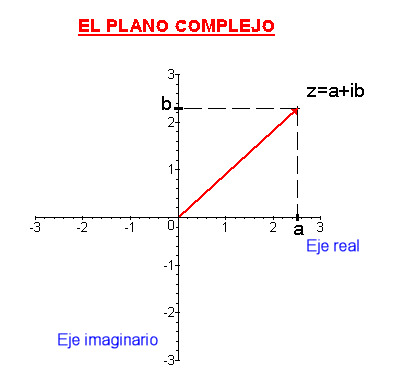
\includegraphics[width=0.5\linewidth]{imagenes/PlanoComplejoRepreGeometrica.jpg}
    \caption{Plano sobre como representar número complejo}
    \label{fig:PlanoComplejo}
\end{figure}

Basándonos en la definición del apartado anterior sobre el inverso y conjugado de un número complejo, al representarlo de forma gráfica queda de la siguiente manera:

\begin{figure}
    \centering
    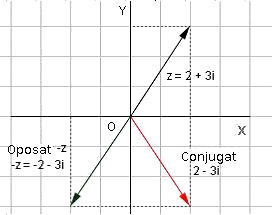
\includegraphics[width=0.5\linewidth]{imagenes/ConjInvCompPlano.jpg}
    \caption{Representación en plano sobre conjugado e inverso}
    \label{fig:ConjInversoPlanoComp}
\end{figure}

\section{Representación forma polar}

Esta representación sirve para destacar los atributos gráficos que tienen los números complejos.\\

\begin{figure}[h]
    \centering
    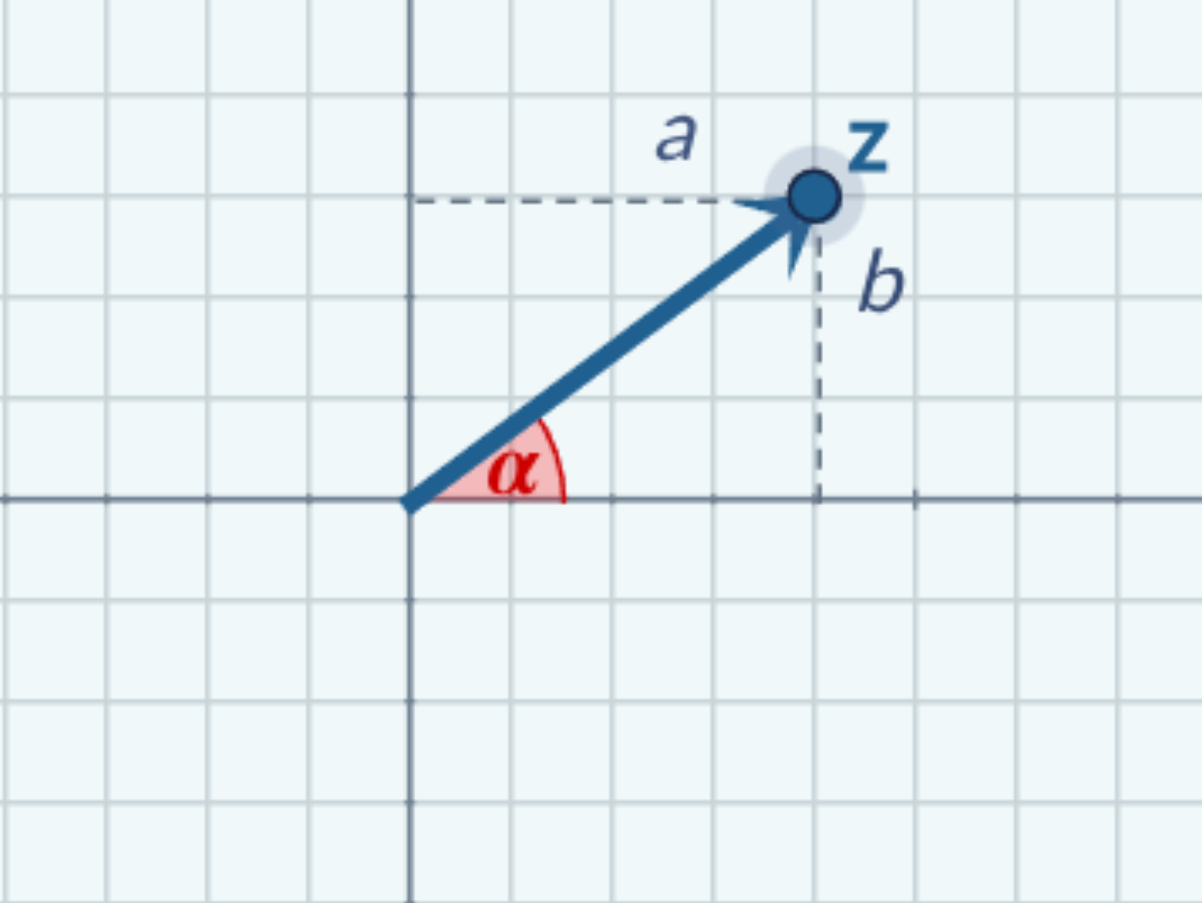
\includegraphics[height=5cm]{imagenes/FormaPolarNumComp.png}
    \caption{Gráfica de la forma polar de un número complejo}
    \label{fig:formaPolar}
\end{figure}

\begin{itemize}
    \item \textbf{Módulo (r):} Distancia del afijo al origen de coordenadas.
    \item \textbf{Argumento (arg(z)):} Ángulo que forma el segmento $\overline{OZ}$ con el semieje positivo medido en el sentido contrario de las agujas del reloj entre 0° y 360°.
\end{itemize}

Con el módulo y el argumento se puede expresar el número complejo \textbf{z} en \textbf{forma polar} de la siguiente forma:
\[
    r_{\alpha} \quad \text{con } r = |z| \text{ y } \alpha = \arg(z)
\]

En base a la forma polar, se puede expresar \textbf{z} en \textbf{forma trigonométrica} de la siguiente manera:

\[
    z = r (\cos \alpha + i \, \sen \alpha), \quad
\]

Esto nos puede servir para pasar de forma polar a forma binómica.\\

\subsection{Operaciones}

Con esta representación, se permite realizar la multiplicación y división de una manera sencilla. Para ello hay que \textbf{expresar los números complejos en forma trigonométrica}.

\begin{itemize}
    \item \textbf{Producto:} $r \cdot r' \, (\cos(\alpha + \beta) + i \, \sen(\alpha + \beta))$\\
          Se observa que el módulo del número complejo es el resultante del producto de los módulos y que el argumento es la suma de los argumentos.

    \item \textbf{Cociente:} $\frac{r}{r'} \, (\cos(\alpha - \beta) + i \, \sen(\alpha - \beta))$
          El resultado del cociente es el cociente de los módulos y la diferencia de los argumentos
\end{itemize}

Por lo que en \textbf{forma polar} quedaría de la siguiente manera:

\begin{itemize}
    \item \textbf{Producto:} $r_\alpha \cdot r_\beta' = (r \cdot r')_{\alpha+\beta}$
    \item \textbf{Cociente:} $\frac{r_\alpha}{r_\beta'} = \left(\frac{r}{r'}\right)_{\alpha - \beta}$
\end{itemize}

Para calcular \textbf{potencia} con exponente natural \textbf{n}, en forma polar, hay que elevar el módulo a \textbf{n} y multiplicar el argumento por \textbf{n}.

\[
    \left( r_\alpha \right)^n = \left( r^n \right)_{n \cdot \alpha}
\]

La \textbf{raíz n-esima} de un número complejo en forma polar, es otro número complejo \textbf{$m_\beta$} que debe de cumplir:

\[
    \left( m_\beta \right)^n = r_\alpha
\]
\[
    m = \sqrt[n]{r} \quad \text{ y } \quad \beta = \frac{\alpha}{n} + \frac{\ang{360} * k}{n}
\]

Todo número complejo tiene n raíces n-ésimas. Todos los afíjos están situados sobre una circunferencia y son los vértices de un polígono regular de n lados. \\

Un ejemplo de forma gráfica calculando la raíz n-esima con lo explicado anterioremnte, es el siguiente:

\newpage
\begin{figure}[h]
    \centering
    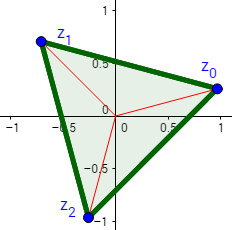
\includegraphics[height=5cm]{imagenes/Raiz3EsimaComplejoPolar.png}
    \caption{Raíz 3-esima del número complejo $z = i + 1$}
    \label{fig:Raiz3esimaComplejo}
\end{figure}

\section{Representación en forma exponencial (Euler)}

El número de Euler ($e$) es un número constante e irracional. Se puede definir a través de la Serie de Taylor.
Este número es la base para resolver ecuaciones relacionadas con el crecimiento exponencial, así como en logaritmos neperianos los cuales sirven para manejar números grandes de una manera simplificada para poder realizar cálculos.\\

La representación del número complejo con el número de Euler, viene dado porque Leonhard Euler aplicó la Serie de Taylor poniéndole la \textbf{$i$} del número imaginario, luego simplificó teniendo en cuenta que \textbf{$i^2 = -1$}. Al aplicar lo comentado, le quedó lo siguiente:

\[
    e^{ix} = \left(1 - \frac{x^2}{2!} + \frac{x^4}{4!} - \dots \right)
    + i \left(x - \frac{x^3}{3!} + \frac{x^5}{5!} - \dots \right)
\] \\

Se dio cuenta que los dos paréntesis de la expresión anterior, es la Serie de Taylor aplicada al \textbf{cos} y \textbf{sen}.

\[
    \cos x = 1 - \frac{x^2}{2!} + \frac{x^4}{4!} - \dots
\]

\[
    \sen x = x - \frac{x^3}{3!} + \frac{x^5}{5!} - \dots
\]\\

Con el seno y coseno, se simplifica en:

\[
    e^{ix} = \cos x + i \, \sen x
\]\\

Este resultado es la representación del número complejo mediante el número de Euler. Además, se le conoce como la \textbf{fórmula de Euler}.

\chapter{Notación Dirac}
\label{chap:notacion_dirac}

La notación de Dirac nos da una manera de expresar estados en un espacio vectorial sin atarnos a un sistema de coordenadas específico, pero que hace muy sencillo elegir una base concreta y cambiar de una base a otra.

\section{Notación bra-ket}

En un \textbf{ket} los valores están representados en un vector columna mientras que en un \textbf{bra} los valores están representados como un vector fila.

\begin{itemize}
    \item \textbf{ket:} Representa un vector con valores complejos, se denota como: $\vec{a} = |a\rangle$
    \item \textbf{bra:} Representa el conjugado del vector complejo ket, se denota como: $\vec{a}^{*} = \langle a|$
\end{itemize}


Para \textbf{realizar la trasformación} entre un \textbf{bra} y un \textbf{ket}, hay que realizar el conjugado de la transpuesta.\\

la base canónica en $\mathbb{C}^2$ viene representado en vector base como $e_1 = (1, 0)$ y $e_2 = (0, 1)$. Por lo que en notación ket quedaría como $|0\rangle = (1, 0)$ y $|1\rangle = (0, 1)$.

\begin{itemize}
    \item \textbf{Producto interno:}  $\langle a|b\rangle = \begin{pmatrix} a_1^{*} & a_2^{*} \end{pmatrix}
                                        \begin{pmatrix} b_1\\ b_2 \end{pmatrix} = a_1^{*} b_1 + a_2^{*} b_2$
    \item \textbf{Producto externo:} $\mathbf{A} = \sum_{i,j=1}^{N} A_{ij}\,|e_i\rangle\langle e_j|
                                      = \sum_{i,j=1}^{N} |e_i\rangle A_{ij} \langle e_j|$
\end{itemize}


\chapter{Qubits}
\label{chap:qubits}

Un \gls{qubit} es el análogo cuántico al bit clásico \cite{ionos_qubits_2023}. Mientras el bit tiene \textbf{dos posibles estados}, el 0 y el 1, el \gls{qubit} se representa como un vector en el espacio vectorial $\mathbb{C}^2$. La base del espacio más utilizada, se denomina base computacional y se corresponde con la base canónica de $\mathbb{C}^2$, que en \textit{notación de Dirac}, son los vectores $\ket{0}$ y $\ket{1}$:

\begin{equation*}
    \begin{array}{rl}
        \ket{0} = & \begin{bmatrix}
                        1 \\ 0
                    \end{bmatrix} \in \mathbb{C}^2 \\
        \ket{1} = & \begin{bmatrix}
                        0 \\ 1
                    \end{bmatrix}
    \end{array}
\end{equation*}

\textbf{Un estado cuántico} es la descripción matemática completa de un sistema cuántico aislado (en este caso, un \gls{qubit}). Más allá de ser un simple vector, este estado encapsula toda la información física y probabilística que podemos conocer del sistema antes de interactuar con él. Dado que se define dentro de un espacio de Hilbert, el estado cuántico obedece al \textit{principio de superposición}, lo que le confiere la capacidad de existir en múltiples configuraciones clásicas de forma simultánea hasta que se produce el colapso mediante una medición.

\section{Expresión del Qubit en Superposición}
Gracias al principio de superposición mencionado anteriormente, un qubit $\ket{\Psi}$ no tiene por qué estar exclusivamente en el estado $\ket{0}$ o en el estado $\ket{1}$. En su lugar, su estado puede ser una \textbf{combinación lineal} de ambos vectores base. A este comportamiento se le denomina \textbf{superposición cuántica}, y permite que el qubit exista como una mezcla simultánea de ambos estados clásicos. En notación de Dirac, esto se representa algebraicamente como:

\[
    \ket{\Psi} = \alpha_0\ket{0} + \alpha_1\ket{1}
\]

Donde $\alpha_0$ y $\alpha_1$ son las \textbf{amplitudes de probabilidad}. De forma general, estas amplitudes se definen como números complejos (lo que, por definición matemática, también incluye a los números reales como un caso particular). Dado que estos coeficientes pueden tomar infinitos valores continuos, un qubit puede adoptar \textbf{infinitos} estados posibles, frente a los únicos dos valores (0 y 1) de un bit clásico. Para que este estado sea válido físicamente, su norma debe ser unitaria, asegurando que la suma de las probabilidades sea 1:

\[
    |\alpha_0|^2 + |\alpha_1|^2 = 1
\]

Cabe destacar que no existe una forma directa de determinar los valores exactos de $\alpha_0$ y $\alpha_1$, ya que el estado cuántico interno no es directamente observable. Antes de realizar una medición, el qubit se encuentra en esta superposición inestable de los estados $\ket{0}$ y $\ket{1}$.

Para conocer el resultado de una computación cuántica, es necesario medir los qubits \cite{sholtis_measure_qubits_2019}. Sin embargo, el acto de medición implica una interacción física que perturba irreversiblemente el sistema. Esto provoca que el qubit abandone su estado de superposición y experimente el \textbf{colapso}. Al colapsar, el qubit se ve forzado a tomar un único valor clásico definido, es decir, pasa a ser estrictamente un $0$ lógico (estado $\ket{0}$) o un $1$ lógico (estado $\ket{1}$). Una vez medido, el qubit se comporta como un bit clásico ordinario, y la información sobre sus amplitudes cuánticas originales se pierde de forma irrecuperable.

La probabilidad exacta de que el qubit colapse hacia un estado u otro está dictada por la \textbf{regla de Born}. Esta regla establece que la probabilidad de observar cada resultado clásico es igual al módulo al cuadrado de su amplitud correspondiente ($P(0) = |\alpha_0|^2$ y $P(1) = |\alpha_1|^2$).

La superposición, tiene distintas representaciones que son:

\begin{itemize}
    \item \textbf{Binómica:} $\ket{\Psi} = (x_0 + i y_0) \ket{0} + (x_1 + i y_1) \ket{1}$
    \item \textbf{Exponencial:} $\ket{\Psi} = r_0 e^{i\phi_0} \ket{0} + r_1 e^{i\phi_1} \ket{1}$
    \item \textbf{Senos y cosenos:} $\ket{\Psi} = \cos\left(\frac{\theta}{2}\right) \ket{0} + e^{i\phi} \sin\left(\frac{\theta}{2}\right) \ket{1}$
\end{itemize}

Existen otros dos conceptos fundamentales relacionados con la superposición y sus fases complejas:

\begin{itemize}
    \item \textbf{Fase global:} Factor común $e^{i\gamma}$ que multiplica a todo el estado $\ket{\Psi}$. Este no cambia ninguna probabilidad ni resultado físico.
    \item \textbf{Fase relativa:} Es la diferencia entre las amplitudes $\alpha$ y $\beta$. Esto influye a las inferencias y los resultados cuando se miden en otras bases $(X, Y)$.
\end{itemize}


\section{Esfera de Bloch}

La esfera de Bloch es una representación visual del estado de un qubit.
Cada punto sobre su superficie corresponde a una posible superposición de los estados base $\ket{0}$ y $\ket{1}$.
Los polos superior e inferior representan los estados $\ket{0}$ y $\ket{1}$, respectivamente, y el estado del qubit se indica con una flecha que apunta hacia el punto que lo describe.

\begin{comment}
\begin{figure}[h]
    \centering
    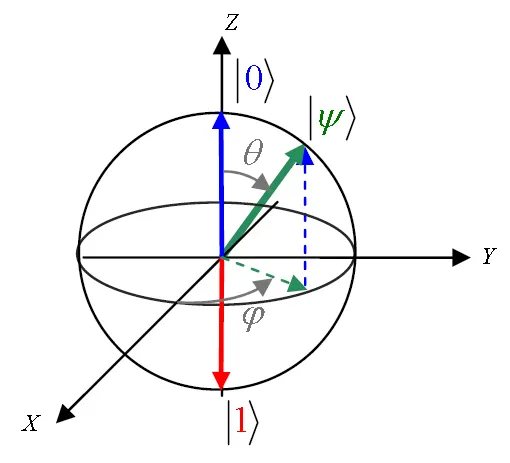
\includegraphics[width=0.5\linewidth]{imagenes/EsferaDeBloch.png}
    \caption{Visualización gráfica esfera de Bloch}
    \label{fig:EsferaDeBloch}
\end{figure}
\newpage

La representación de la esfera de Bloch de la imgaen, se le conoce como \textbf{ejes de Pauli}. Como tiene ángulos, se utiliza la representación de coordenadas esféricas principalmente. En dicha representación, se proporciona los dos ángulos y la longitud que viene denotado como $(r, \theta,\phi)$
donde $r$ es la longitud y $\theta$ y $\phi$ representan el ángulo del eje Z positivo con el de X positivo en el plano X-Z y el angulo entre el eje positivo X y el eje positivo Y del plano X-Y respectivamente
\end{comment}

\begin{figure}[h]
    \centering
    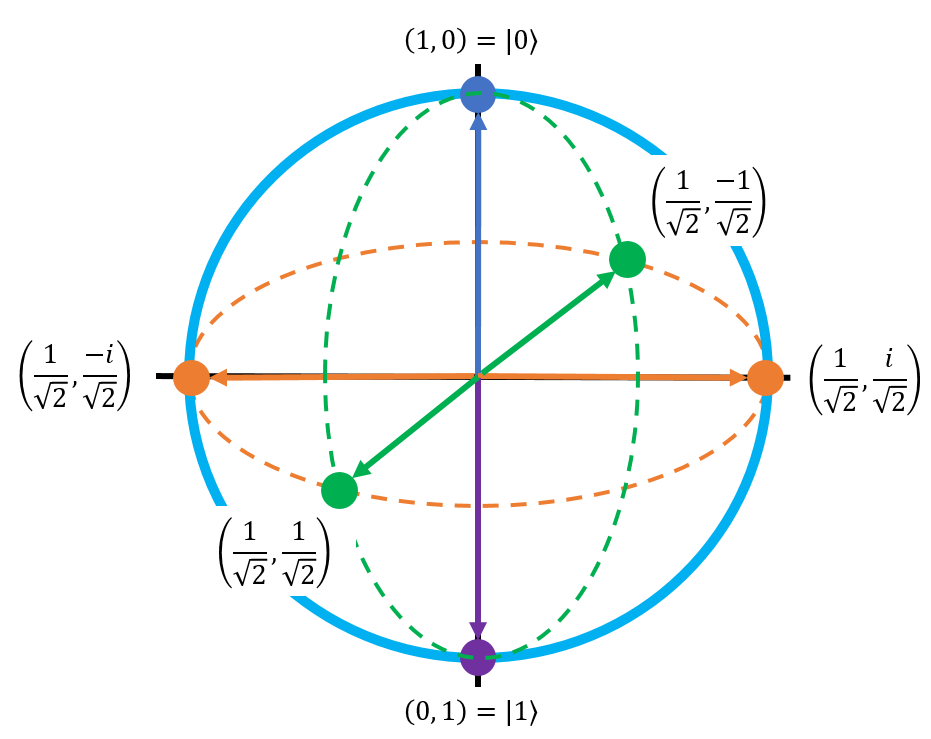
\includegraphics[width=0.5\linewidth]{imagenes/bloch-basic.png}
    \caption{Visualización gráfica de la esfera de Bloch. Imagen obtenida de \cite{mitre_bloch_sphere_2022}}
    \label{fig:EsferaDeBloch}
\end{figure}
\newpage

\textbf{Importante:} la notación $\left(\frac{1}{\sqrt{2}}, \frac{1}{\sqrt{2}}\right)$ se corresponde con el vector estado $\begin{bmatrix} \frac{1}{\sqrt{2}} \\ \frac{1}{\sqrt{2}} \end{bmatrix}$ que a su vez significa:

\[
    \begin{bmatrix} \frac{1}{\sqrt{2}} \\ \frac{1}{\sqrt{2}} \end{bmatrix} = \frac{1}{\sqrt{2}}|0\rangle + \frac{1}{\sqrt{2}}|1\rangle
\]

Los seis puntos principales de la esfera de Bloch son los que se ve en la Figura \ref{fig:EsferaDeBloch} \cite{castano_qubit_bloch_2025}. A estas coordenadas principales se le pueden asignar etiquetas.

\begin{itemize}
    \item \textbf{Base de Hadamard:} También se le conoce como eje X de Pauli. El punto $\left(\frac{1}{\sqrt{2}}, \frac{1}{\sqrt{2}}\right)$ se corresponde con $\ket{+}$. A su vez, el punto opuesto $\left(\frac{1}{\sqrt{2}}, \frac{-1}{\sqrt{2}}\right)$ se corresponde con $\ket{-}$

    \item \textbf{Base circular:} También se le conoce como eje Y de Pauli. El punto $\left(\frac{1}{\sqrt{2}}, \frac{i}{\sqrt{2}}\right)$ se corresponde con $\ket{+i}$. A su vez, el punto opuesto $\left(\frac{1}{\sqrt{2}}, \frac{-i}{\sqrt{2}}\right)$ se corresponde con $\ket{-i}$
\end{itemize}

Con dicha asignación de etiquetas, queda la esfera que se muestra en la Figura \ref{fig:EsferaDeBlochReducido}:

\begin{figure}[h]
    \centering
    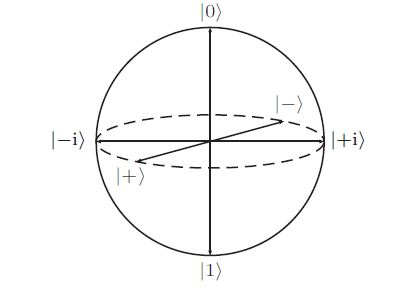
\includegraphics[width=0.5\linewidth]{imagenes/bloch-labels.jpg}
    \caption{Imagen obtenida de \url{https://en.wikipedia.org/wiki/Bloch_sphere}}
    \label{fig:EsferaDeBlochReducido}
\end{figure}
\newpage

\section{Puertas cuánticas}

Al igual que para manipular los valores de los bits existen puertas lógicas clásicas como OR, AND, NOT, etc. Los ordenadores cuánticos manipulan los valores de los qubits usando puertas cuánticas \cite{spinq_quantum_gates_2025}. Esto implica que cualquier algoritmo cuántico se tiene que implementar usando puertas cuánticas.

Las puertas cuánticas se \textbf{representan} matemáticamente mediante \textbf{matrices unitarias} $U$ \cite{gopalan_module3_2022}. Una matriz se considera unitaria si, al multiplicarla por su adjunta o conjugada transpuesta ($U^{\dagger}$), el resultado es la matriz identidad ($U^{\dagger}U = U U^{\dagger} = I$). Esta propiedad matemática es fundamental porque garantiza que la transformación es \textbf{reversible} y preserva la norma de los vectores. Esto significa que la puerta cuántica conserva siempre la probabilidad total de todos los posibles resultados, por lo que no se destruye ni se pierde información cuántica durante la operación.

Al aplicar una puerta cuántica $U$ a un estado cuántico $\ket{\psi}$ se realiza la multiplicación matricial $\ket{\psi'} = U \ket{\psi}$. Si expresamos el nuevo estado resultante como $\ket{\psi'} = \alpha_0' \ket{0} + \alpha_1' \ket{1}$, la propiedad unitaria asegura que la norma siga siendo unitaria. Es decir, independientemente de la puerta cuántica que se aplique, la regla de conservación de probabilidad se mantiene intacta: $|\alpha_0'|^2 + |\alpha_1'|^2 = 1$.

Poniendo un ejemplo sencillo, consideremos la puerta Pauli-X (el análogo cuántico de la puerta NOT clásica), cuya matriz unitaria es $X = \begin{pmatrix} 0 & 1 \\ 1 & 0 \end{pmatrix}$. Si aplicamos esta puerta sobre el estado base $\ket{0}$, el estado transiciona a $\ket{1}$:

\[
    X \ket{0} = \begin{pmatrix} 0 & 1 \\ 1 & 0 \end{pmatrix} \begin{pmatrix} 1 \\ 0 \end{pmatrix} = \begin{pmatrix} 0 \\ 1 \end{pmatrix} = \ket{1}
\]

Como $X$ es una matriz unitaria (y resulta ser su propia inversa, $X^{\dagger}X = I$), la operación es completamente reversible. Si aplicamos $X$ por segunda vez, recuperamos matemáticamente el estado original $\ket{0}$ sin perder ninguna información en el proceso:

\[
    X (X \ket{0}) = X \ket{1} = \begin{pmatrix} 0 & 1 \\ 1 & 0 \end{pmatrix} \begin{pmatrix} 0 \\ 1 \end{pmatrix} = \begin{pmatrix} 1 \\ 0 \end{pmatrix} = \ket{0}
\]

Las puertas cuánticas para un único qubit son:

\begin{itemize}
    \item \textbf{Pauli I (Identidad):} Se considera la operación trivial o identidad. Su función es dejar el qubit inalterado, y su operador asociado se denota mediante la matriz identidad $I$:
          \[
              I = \begin{bmatrix}
                  1 & 0 \\
                  0 & 1
              \end{bmatrix}
          \]

    \item \textbf{Pauli X:} Conocida coloquialmente como la puerta NOT cuántica. Algebraicamente se define por la siguiente matriz:
          \[
              X = \begin{bmatrix}
                  0 & 1 \\
                  1 & 0
              \end{bmatrix}
          \]

          Al aplicar esta puerta, las amplitudes de probabilidad se intercambian, lo que provoca que los estados base $\ket{0}$ y $\ket{1}$ se inviertan.

    \item \textbf{Pauli Y:} Esta transformación combina una inversión de los estados con un cambio de fase complejo. Su estructura viene dada por:
          \[
              Y = \begin{bmatrix}
                  0 & -i \\
                  i & 0
              \end{bmatrix}
          \]

          Si un qubit en superposición $\ket{\psi} = \alpha_0\ket{0} + \alpha_1\ket{1}$ atraviesa esta puerta, el efecto resultante es:
          \[
              Y\ket{\psi} = \begin{bmatrix} 0 & -i \\ i & 0 \end{bmatrix} \begin{bmatrix} \alpha_0 \\ \alpha_1 \end{bmatrix} = \begin{bmatrix} -i\alpha_1 \\ i\alpha_0 \end{bmatrix} = -i\alpha_1\ket{0} + i\alpha_0\ket{1}
          \]

    \item \textbf{Pauli Z:} Actúa modificando únicamente la fase del estado $\ket{1}$ (añadiendo un desfase de $\pi$). Su operador matricial se expresa como:
          \[
              Z = \begin{bmatrix}
                  1 & 0  \\
                  0 & -1
              \end{bmatrix}
          \]

          Matemáticamente, al operar sobre un qubit genérico $\ket{\psi} = \alpha_0\ket{0} + \alpha_1\ket{1}$, altera exclusivamente el signo de la segunda amplitud:
          \[
              Z\ket{\psi} = \begin{bmatrix} 1 & 0 \\ 0 & -1 \end{bmatrix} \begin{bmatrix} \alpha_0 \\ \alpha_1 \end{bmatrix} = \begin{bmatrix} \alpha_0 \\ -\alpha_1 \end{bmatrix} = \alpha_0\ket{0} - \alpha_1\ket{1}
          \]

    \item \textbf{Puerta Hadamard (H):} Es una de las operaciones más fundamentales, ya que al aplicarse sobre un estado base puro genera una superposición equitativa. Se define matricialmente como:
          \[
              H = \frac{1}{\sqrt{2}}\begin{bmatrix}
                  1 & 1  \\
                  1 & -1
              \end{bmatrix}
          \]

          Si aplicamos esta transformación a un estado en superposición $\ket{\psi} = \alpha_0\ket{0} + \alpha_1\ket{1}$, las amplitudes se mezclan obteniendo la siguiente salida:
          \[
              H\ket{\psi} = \frac{1}{\sqrt{2}}\begin{bmatrix} 1 & 1 \\ 1 & -1 \end{bmatrix} \begin{bmatrix} \alpha_0 \\ \alpha_1 \end{bmatrix} = \frac{1}{\sqrt{2}}\begin{bmatrix} \alpha_0 + \alpha_1 \\ \alpha_0 - \alpha_1 \end{bmatrix} = \left(\frac{\alpha_0 + \alpha_1}{\sqrt{2}}\right)\ket{0} + \left(\frac{\alpha_0 - \alpha_1}{\sqrt{2}}\right)\ket{1}
          \]
\end{itemize}

\chapter{Procesamiento Lenguaje Natural}
\label{chap:pln}

\section{Introducción al Procesamiento del Lenguaje Natural}

El \acrfull{pln} es la rama de la \gls{ia} encargada de la interacción entre computadoras y el lenguaje humano. Este campo integra la lingüística computacional, basada en el modelado de reglas del lenguaje, con modelos estadísticos y algoritmos de aprendizaje profundo (\gls{dl}) y aprendizaje automático (\gls{ml}) \cite{stryker_what_nlp}.

El \gls{pln} forma parte a día de hoy de muchos motores de búsqueda, chatbots para atención al cliente (ya sea por escrito o por voz), y asistentes digitales como Alexa de Amazon o Siri de Apple.

El campo de la computación lingüística incluye tradicionalmente diversas fases para el análisis. Para el análisis de las palabras existen dos enfoques principales:

\begin{itemize}
      \item \textbf{Análisis de dependencias:} Examina las relaciones gramaticales binarias entre las palabras, identificando, por ejemplo, qué palabra modifica a cuál o cuál es el sujeto y el verbo principal.

      \item \textbf{Análisis de constituyentes:} Construye un árbol sintáctico que representa la estructura gramatical anidada de una oración, descomponiéndola en sintagmas o frases ordenadas jerárquicamente.
\end{itemize}

\section{Fases del \glsentryshort{pln}}

Las fases para realizar el \gls{pln} se pueden observar en la Figura \ref{fig:FasesNLP}:

\begin{figure}[h]
      \centering
      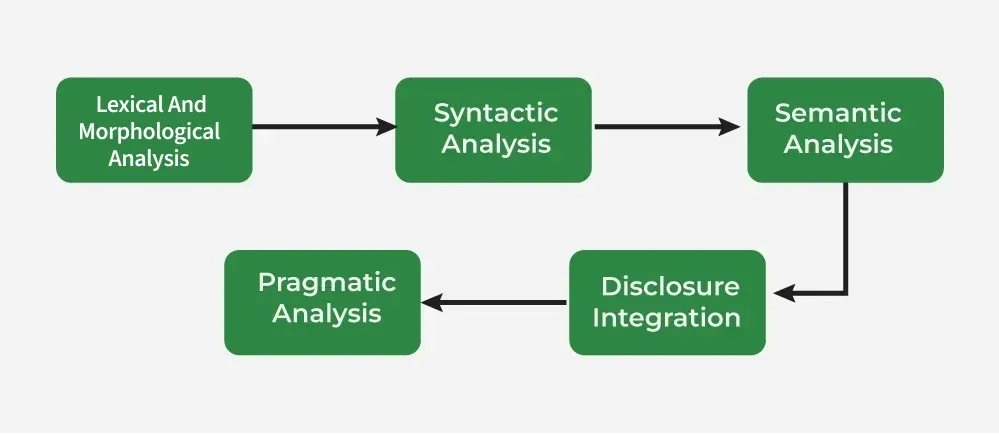
\includegraphics[width=1.0\linewidth]{imagenes/FasesNLP.png}
      \caption{Esquema de las fases del \gls{pln}. Extraído de \cite{geeksforgeeks_phases_nlp_2025}.}
      \label{fig:FasesNLP}
\end{figure}

A continuación, basándose en la estructura descrita en \cite{geeksforgeeks_phases_nlp_2025}, se detalla en qué consiste cada una de estas fases:

\subsection{Preprocesamiento y Tokenización}

Esta fase constituye el nivel inicial del procesamiento lingüístico computacional. Su propósito fundamental es transformar el texto crudo en una secuencia estructurada de unidades discretas y manejables. Para lograrlo, se integran diversas tareas de análisis léxico y morfológico que preparan la información para las etapas posteriores.

\begin{enumerate}
      \item \textbf{Preprocesamiento:} Esta fase inicial comprende un conjunto de operaciones destinadas a homogeneizar el texto. Entre las principales subtareas se encuentran la limpieza del contenido, la normalización (como la conversión a minúsculas) y la eliminación de caracteres especiales. Adicionalmente, suele llevarse a cabo la supresión de las \textit{stopwords}, que son palabras de muy alta frecuencia pero que carecen de una gran carga semántica (tales como ``el'', ``de'', ``y''). Como parte de este preprocesamiento, también se aplican técnicas de análisis morfológico para estandarizar el vocabulario:
            \begin{itemize}
                  \item \textit{Lematización:} Consiste en convertir las palabras a su forma base o lema canónico (por ejemplo, el verbo ``soy'' se transforma en ``ser'').
                  \item \textit{Stemming:} Se basa en reducir las palabras a su raíz léxica, eliminando sufijos y prefijos (por ejemplo, ``niñero'' se reduce a ``niño'').
            \end{itemize}

      \item \textbf{Tokenización:} Representa el proceso crítico mediante el cual se segmenta el flujo de texto en unidades atómicas significativas, denominadas \textit{tokens}.

            A modo de ejemplo, la oración \textit{Me gusta programar} se dividiría en la siguiente lista de tokens: \texttt{[``Me'', ``gusta'', ``programar'']}.

            La granularidad de los tokens depende del modelo empleado. Pueden corresponder a palabras completas, subpalabras (una técnica común en los modelos de tipo \gls{gpt}) o incluso a caracteres individuales. Una vez completada la tokenización, a cada token se le asigna un índice numérico único dentro de un vocabulario, un paso indispensable para la posterior generación de representaciones vectoriales o \textit{Embeddings} (concepto que se desarrollará en detalle en el Capítulo \ref{chap:word_embeddings}).

      \item \textbf{Etiquetado gramatical (\gls{pos} Tagging):} En esta etapa se asigna a cada token su correspondiente categoría morfológica (como sustantivo, verbo, adjetivo, entre otras), tomando en consideración tanto su definición formal como el contexto en el que aparece. Esto resulta esencial para desambiguar la función sintáctica que desempeña cada palabra en la oración.

            Siguiendo con el ejemplo anterior, el etiquetado de los tokens daría como resultado: \texttt{[``Me'' $\rightarrow$ Pronombre, ``gusta'' $\rightarrow$ Verbo, ``programar'' $\rightarrow$ Verbo]}.
\end{enumerate}

\subsection{Análisis sintáctico}

El análisis sintáctico examina la organización de las palabras dentro de una oración para verificar que se cumple con las reglas gramaticales del idioma. El objetivo fundamental de esta fase es la generación de un \textbf{árbol de análisis sintáctico}, el cual representa jerárquicamente la estructura gramatical del texto analizado. Esta representación estructurada permite a los sistemas computacionales interpretar las relaciones de dependencia y jerarquía entre los distintos elementos léxicos. Las tareas principales que abarca son:

\begin{itemize}
      \item \textbf{Etiquetado gramatical:} Se fundamenta en el proceso de \gls{pos} Tagging explicado en la fase de \textit{Preprocesamiento y Tokenización}. En esta etapa de análisis sintáctico, las categorías morfológicas previamente asignadas a cada token se utilizan para validar la corrección de la estructura jerárquica de la oración.
      \item \textbf{Resolución de ambigüedad sintáctica:} Consiste en determinar la estructura gramatical correcta cuando una oración puede analizarse de múltiples formas. Por ejemplo, en la frase \textit{Vi al hombre con el telescopio}, el sistema debe resolver si el telescopio es el instrumento utilizado por el sujeto para ver, o si es un objeto que lleva consigo el hombre.
\end{itemize}

\subsection{Análisis semántico}

Esta fase se centra en la coherencia lógica y la relevancia contextual del enunciado. Su objetivo principal es interpretar el significado de las palabras, analizando tanto su definición de diccionario como su variación según el contexto de uso. De este modo, se busca comprender el rol semántico de cada palabra para construir una representación lógica del mensaje. Las tareas fundamentales que abarca esta fase son:

\begin{enumerate}
      \item \textbf{\gls{ner}:} Se ocupa de la identificación y clasificación de elementos clave en el texto, tales como nombres de personas, ubicaciones geográficas, organizaciones, etc.
            \\
            Ejemplo: En la oración \textit{Mercedes anunció un nuevo coche en Berlín}, el sistema \gls{ner} identificaría a \textit{Mercedes} como una \textit{Organización} y a \textit{Berlín} como un \textit{Lugar}.

      \item \textbf{\gls{wsd}:} Consiste en identificar el significado exacto de una palabra polisémica basándose en el contexto en el que se encuentra (proceso conocido como resolución de ambigüedad léxico-semántica).
            \\
            Ejemplo: El término \textit{banco} se interpreta como una \textit{entidad financiera} en la frase \textit{Fui a sacar dinero al banco}, pero adquiere el significado de \textit{asiento} en la oración \textit{Me senté en el banco del parque}.
\end{enumerate}

\subsection{Integración del discurso}

Este proceso analiza cómo las oraciones individuales se conectan y relacionan entre sí para entender el contexto global. El objetivo de esta fase es garantizar que el significado del texto mantenga su coherencia lógica a través de los distintos párrafos y frases. Los aspectos fundamentales de esta fase son:

\begin{itemize}
      \item \textbf{Resolución de anáforas:} Consiste en identificar la conexión entre un pronombre y lo mencionado previamente en el texto.
            \\
            Ejemplo: En la secuencia \textit{Esther fue a comprar. Ella compró fruta}, el sistema debe vincular el pronombre \textit{Ella} con \textit{Esther}.

      \item \textbf{Referencias contextuales:} Aborda la interpretación de palabras o expresiones cuyo significado completo depende intrínsecamente de la información proporcionada en oraciones anteriores o posteriores.
            \\
            Ejemplo: La frase \textit{Fue un buen día} adquiere un significado concreto únicamente si se analiza dentro del contexto de la conversación.
\end{itemize}

\subsection{Análisis pragmático}

Esta fase final analiza más allá de la interpretación literal de las oraciones para inferir el significado real que se pretende transmitir. A diferencia del análisis semántico, que se ocupa del significado proposicional de las palabras, el análisis pragmático examina factores como el tono y el contexto. Las tareas principales de esta fase son:

\begin{itemize}
      \item \textbf{Detección de intenciones:} El sistema debe ver el propósito de la comunicación (si es una petición, una queja, una orden, etc.).
            \\
            Ejemplo: Ante la pregunta \textit{¿Tienes hora?}, el análisis pragmático entiende que la intención real del usuario es saber qué hora es, no una pregunta de sí o no.

      \item \textbf{Interpretación de lenguaje figurado:} Se encarga de identificar metáforas, ironías o frases hechas.
            \\
            Ejemplo: En la expresión \textit{Echar una mano}, el análisis pragmático entiende que significa \textit{ayudar a alguien}.
\end{itemize}



\chapter{Procesamiento del Lenguaje Natural Cuántico (\glsentrytext{qnlp})}

\section{Motivación para el uso de \glsentrytext{qnlp}}

Tal y como se expuso en el capítulo precedente, la implementación del \glsentrytext{nlp} mediante técnicas de \glsentrytext{dl} ha representado un gran avance. Sin embargo, estos modelos enfrentan desafíos significativos, principalmente el elevado coste computacional y de memoria.

La teoría cuántica ofrece nuevos paradigmas para el modelado matemático y la computación. Se han desarrollado modelos inspirados en la mecánica cuántica para abordar tareas complejas como la recuperación de información y la desambiguación semántica.

Adicionalmente, en el ámbito del \glsentrytext{ml}, se ha demostrado teóricamente que los modelos cuánticos de \glsentrytext{ml} (\glsentrytext{qml}) presentan una capacidad de expresividad superior a la de los modelos clásicos en ciertos regímenes, haciendo que sea un foco de estudio actual para la mejora de los modelos \glsentrytext{nlp}. El \glsentrytext{qnlp} busca explotar ventajas cuánticas como el paralelismo y la alta dimensionalidad del espacio de estados para procesar lenguaje de manera más eficiente o con mayor riqueza semántica.

\section{Paralelismo entre Espacio Semántico y Espacio de Hilbert}

\section{Codificación de información clásica en estados cuánticos}

\subsection{Basis Encoding y Amplitude Encoding}

\section{Circuitos Cuánticos Variacionales (\glsentrytext{vqc}) como modelos de aprendizaje}

\chapter{Representación Vectorial de Palabras (Word Embeddings)}


\section{Introducción al concepto de \textit{Embedding}}

De manera intuitiva, un \textit{embedding} de texto es una representación matemática que proyecta un fragmento de texto en un espacio latente de alta dimensionalidad. En este espacio, la posición del texto se define mediante un vector, donde cada componente del vector corresponde a una dimensión. Al igual que en un plano cartesiano se tienen dos dimensiones, en un embedding, se suele trabajar con muchas más dimensiones para representar una palabra en el espacio\cite{henner_intuitive_embeddings_2023}. Por ejemplo, el modelo de \textbf{OpenAI} \textit{text-embedding-ada-002} el cual tiene un espacio de dimensión de 1536. Es decir, cada vector está formado por 1536 componentes.

Un ejemplo de cómo se verían los valores que toma cada dimensión es el siguiente:

\begin{quote}
  \textit{``A text embedding is a piece of text projected into a high-dimensional latent space. The position of our text in this space is a vector, a long sequence of numbers. Think of the two-dimensional cartesian coordinates from algebra class, but with more dimensions---often 768 or 1536.''} \cite{henner_intuitive_embeddings_2023}
\end{quote}

Al procesar el párrafo anterior mediante el modelo \textit{text-embedding-ada-002} mencionado, se obtiene la gráfica de la Figura \ref{fig:ejemploValoresEmbedding}, donde cada barra vertical representa el valor asignado a una de sus 1536 dimensiones.

\begin{figure}[h]
  \centering
  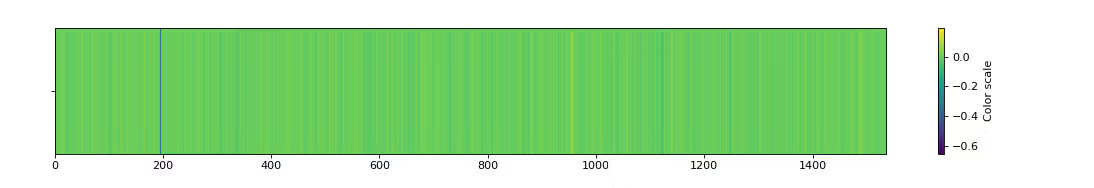
\includegraphics[width=0.8\linewidth]{imagenes/ejemploValoresEmbedding.png}
  \caption{Representación gráfica de los valores en las 1536 dimensiones de un embedding generado por el modelo text-embedding-ada-002. Fuente: \cite{henner_intuitive_embeddings_2023}.}
  \label{fig:ejemploValoresEmbedding}
\end{figure}

Un \textbf{espacio de embedding} o \textbf{espacio latente} se define matemáticamente como un espacio donde los elementos están posicionados de manera más cercana uno del otro cuando tienen valores parecidos, mientras que si difieren dichos elementos, se posicionan más lejos entre ellos. En el caso del \glsentrytext{pln}, frases que son semánticamente más similares a otras, tendrán un vector de embedding similar por lo que estarán más juntas en el espacio.

Aunque la comparación entre frases es una de las aplicaciones más conocidas, los \textit{embeddings} también se aplica en modelos de \glsentrytext{ml} y en arquitecturas de redes neuronales complejas.

\subsection{Embeddings de palabras (\textit{Word Embeddings})}

Mientras que el concepto general de \textit{embedding} puede aplicarse a frases completas (como en el ejemplo introducido), su uso más extendido e histórico se encuentra en su aplicación a nivel atómico: las palabras. Un \textit{embedding} de palabras, es un vector de longitud fija el cual su único cometido, es representar una única palabra o \textit{token} \cite{almeida_word_2023}.

El diseño y creación de estos vectores se clasifica principalmente en dos grandes familias estratégicas, dependientes de sus algoritmos de generación: los \textbf{modelos basados en predicciones} y los \textbf{modelos basados en conteos}.

\subsubsection{Modelos basados en predicciones}

Esta técnica de representación surgió fuertemente ligada al desarrollo de los \glsentryplural{mnl}. A diferencia de los enfoques estadísticos tradicionales de recuento, un modelo predictivo se centra en aprender el significado de un término de forma prospectiva, es decir, "adivinando".

Para lograrlo, emplean una red neuronal sencilla dotada de una ventana de contexto de tamaño fijo y móvil (por ejemplo, avanzando de cinco en cinco palabras). A medida que lee el texto, el modelo intenta predecir el significado de una palabra central en base a las palabras vecinas de esta ventana, o a la inversa, predecir el contexto apoyándose únicamente en dicho término central.

El aspecto fundamental en todo esto, es que tras finalizar el entrenamiento, el objetivo de \glsentrytext{ml} deja de ser la capacidad del modelo para adivinar con exactitud. En su lugar, de la red neuronal, se extraen los \textbf{pesos y valores} que ha ajustado internamente. Estos valores que fueron ajustados durante el entrenamiento, se convierten directamente en el \textit{word embedding}. En consecuencia, el mecanismo iterativo garantiza que aquellas palabras empleadas en contextos idénticos acaben reteniendo representaciones vectoriales prácticamente iguales.

\begin{figure}[h]
  \centering
  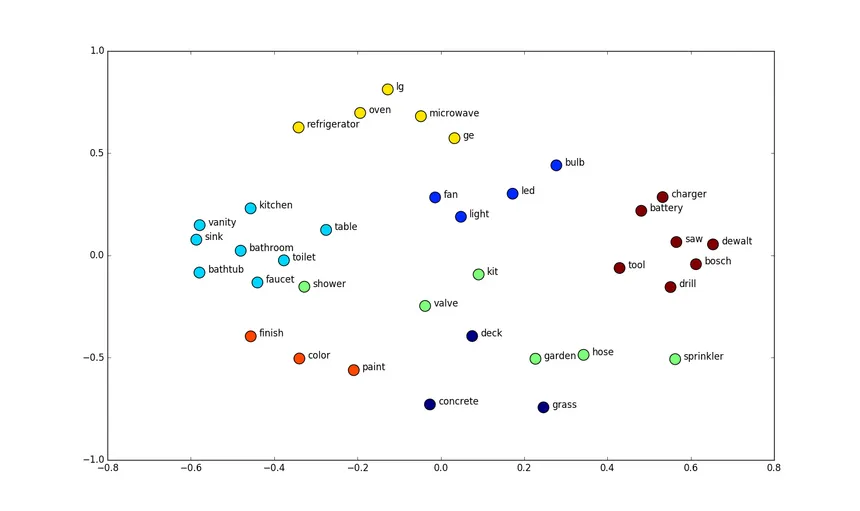
\includegraphics[width=0.8\linewidth]{imagenes/Word-embeddings-model.png}
  \caption{Representación visual de un modelo basado en predicciones para generar embeddings de palabras. Fuente: \url{https://neptune.ai/blog/word-embeddings-guide}.}
  \label{fig:word_embeddings_model}
\end{figure}

Una de las arquitecturas más representativas dentro de la predicción de \textit{embeddings} es la famosa familia algorítmica \textbf{Word2Vec}, la cual se detalla de forma exhaustiva en el próximo capítulo.

\subsubsection{Modelos basados en conteos}

Por su parte, la segunda categoría de modelos hace uso de la estadística global a lo largo de un documento completo (\textit{corpus}). Estos modelos se aprovechan de los recuentos de coocurrencia (palabra y contexto) estructurando toda la información como grandes \textit{matrices de palabra-contexto}.

El funcionamiento radica en la creación de una matriz gigantesca donde se contabiliza el número de apariciones conjuntas en las que una palabra acompaña a todo un posible contexto del propio texto. No obstante, si el conjunto de datos cuenta con $n$ palabras distintas, las dimensiones de la matriz ascenderán a un total de $n \times n$. Esto acarrea severamente un cuello de botella de almacenamiento. Adicionalmente, la inmensa mayoría de cruces de dicha matriz representarán palabras que jamás han coexistido en el texto (por ejemplo, "oveja" y "pantalla"), llenando de ceros el modelo de datos. Esta estructura tan ineficiente es conocida como \textbf{matriz dispersa}.

Para solventar esta carencia y la falta de memoria, se reduce la dimensionalidad a través de complejas operaciones de álgebra lineal, como puede ser la \gls{dvs}. Con esto logran sintetizar enormes matrices de ceros, transformándolos en \textbf{vectores cortos y densos}. De tal modo, que los conceptos globalmente equivalentes retengan valores numéricamente similares sin desperdiciar memoria.

La \textbf{mayor ventaja} de esta táctica estadística contable, frente al sistema predictivo, reside precisamente en que es capaz de aprovechar la información global de todo el \textit{corpus}, un aspecto estadístico que se le escapa a las ventanas de lectura en las redes neuronales por definición.

El modelo híbrido con más popularidad en este ámbito es el de \textbf{GloVe (\textit{Global Vectors})}. Desarrollado por un equipo de investigadores de la Universidad de Stanford, logra exitosamente agrupar los beneficios numéricos de las matrices grandes de conteo global, con las altas capacidades de optimización paramétrica propias de los modelos del \glsentrytext{ml}.

\begin{figure}[h]
  \centering
  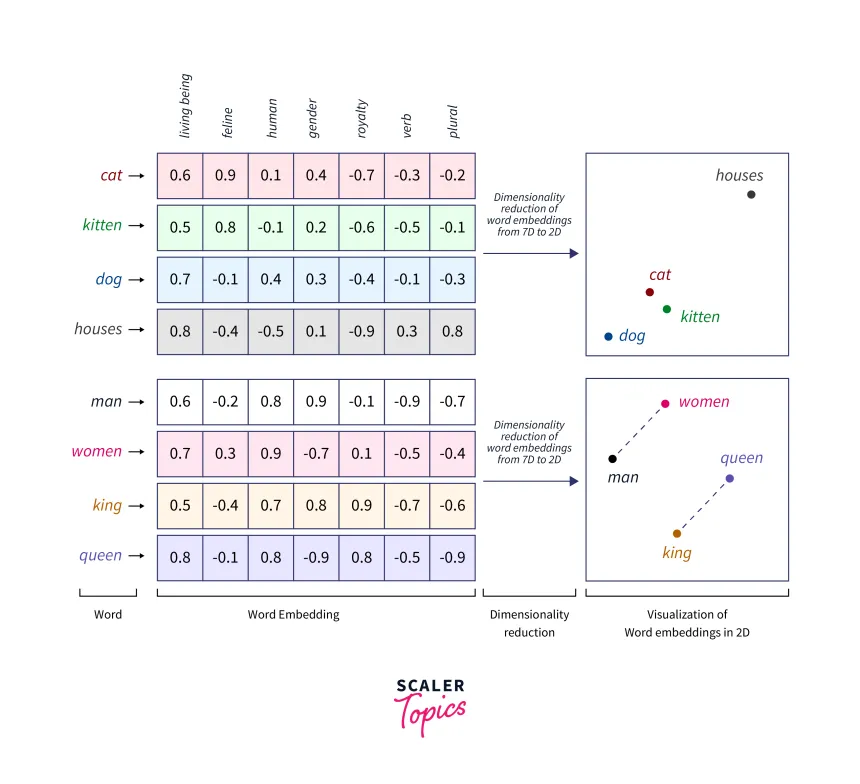
\includegraphics[width=0.8\linewidth]{imagenes/word-embedding-counting-model.png}
  \caption{Representación visual de un modelo basado en conteos para generar embeddings de palabras. Fuente: \url{https://www.scaler.com/topics/tensorflow/tensorflow-word-embeddings/}.}
  \label{fig:word_embedding_counting_model}
\end{figure}

\section{Espacios vectoriales y similitud semántica}

El espacio semántico \cite{worth_word_embeddings_2023} se define geométrica y algebraicamente como un espacio de $N$ dimensiones, donde $N$ representa el número de características. En las aplicaciones de aprendizaje automático para el \glsentrytext{pln}, estas características son típicamente palabras, n-gramas o frases completas.

Este espacio acota matemáticamente tanto el dominio del problema como el dominio de la solución. En el caso particular de los \textit{word embeddings}, las dimensiones son aprendidas por el propio modelo para asegurar que este exhiba ciertas propiedades; propiedades que son función de lo que se conoce como la \textbf{hipótesis distribucional}.

La hipótesis distribucional establece que las palabras que aparecen en contextos similares tienden a tener significados análogos. Para que el espacio vectorial refleje geométricamente esta propiedad sin que colapse analíticamente por culpa de tener miles o millones de características, no basta con usar métricas simples como el recuento de palabras. Es necesario transformar los datos basándose en el uso de \textbf{información latente}, logrando destilar el significado abstracto en unos pocos ejes temáticos.

Una vez que las palabras se han convertido en vectores y se han posicionado en este espacio latente optimizado, el siguiente paso natural es medir qué tan afines son sus significados. Esta similitud semántica se traduce matemáticamente en calcular la \textbf{distancia} geométrica que separa a ambos vectores.

A continuación, se detallan estos dos principios fundamentales para el funcionamiento profundo de los \textit{embeddings}.

\subsection{Información Latente}

% Aquí puedes adaptar la parte del texto que hablaba de "Latent information" (pasar del bag-of-words con perro/gato a los ejes latentes como "feline" o "mamífero")


\subsection{Métricas de Distancia}

% Aquí puedes adaptar la parte del texto de "Distance" (explicar la limitación de la distancia euclídea y por qué se normaliza con la distancia coseno)


\section{Paralelismo entre Espacio Semántico y Espacio de Hilbert}

Existe una analogía natural entre el espacio semántico clásico y el formalismo matemático de la mecánica cuántica.

En el \glsentrytext{pln} clásico, modelamos el significado de las palabras mapeándolas a vectores en un espacio vectorial real ($\mathbb{R}^n$). En la computación cuántica, operamos con estados cuánticos que "habitan" en un espacio vectorial complejo con producto interno, conocido formalmente como **Espacio de Hilbert** ($\mathcal{H}$).

Mientras que el espacio semántico clásico asigna vectores de características fijas, el Espacio de Hilbert ofrece un marco matemático mucho más rico. Los estados cuánticos en este espacio pueden existir en superposición y estar entrelazados, propiedades fundamentales que permiten representar la ambigüedad y la composición del lenguaje de una manera que los espacios vectoriales clásicos no pueden replicar eficientemente.

En el contexto del \glsentrytext{plnc}, la propuesta es mapear las palabras no a simples vectores reales, sino a estados cuánticos dentro de este Espacio de Hilbert. Esto permite que la gramática y el significado se combinen utilizando operaciones tensoriales y evolución unitaria, aprovechando la estructura exponencial del espacio de estados cuánticos para procesar el lenguaje.

\chapter{Implementación Clásica: Algoritmo Word2Vec}

Word2Vec, cuyo nombre proviene de la contracción de \textit{Word to Vector}, es un modelo de \glsentrytext{ml} que permite representar palabras como vectores de grandes dimensiones. Su principal virtud reside en que las relaciones semánticas y sintácticas entre palabras quedan codificadas como proximidad geométrica entre dichos vectores, permitiendo así capturar el significado de forma numérica y operable.

Fue desarrollado y publicado por Google en 2013 \cite{google_word2vec_2013}, además en esa misma fecha, se introdujo este modelo en su motor de búsqueda. Desde entonces, el modelo ha sido ampliamente adoptado y ha dado lugar a múltiples mejoras y variantes de rendimiento.

En este capítulo se explorarán la arquitectura del modelo, su función de optimización y el proceso de entrenamiento que permite generar el espacio vectorial latente en el que las palabras quedan representadas.

\section{Arquitectura del modelo}

Word2Vec aprende las representaciones de las palabras procesando grandes volúmenes de texto y capturando el contexto en el que aparece cada término \cite{logunova_word2vec_serokell}. Su arquitectura se fundamenta en una red neuronal superficial (\textit{shallow neural network}), que a diferencia de las redes profundas (\textit{deep neural networks}), dispone únicamente de una capa oculta entre la capa de entrada y la de salida. Este diseño proporciona una ventaja clave: permite entrenar el modelo de forma eficiente sobre corpus de gran tamaño, manteniendo un coste computacional razonable.

\begin{figure}[h]
  \centering
  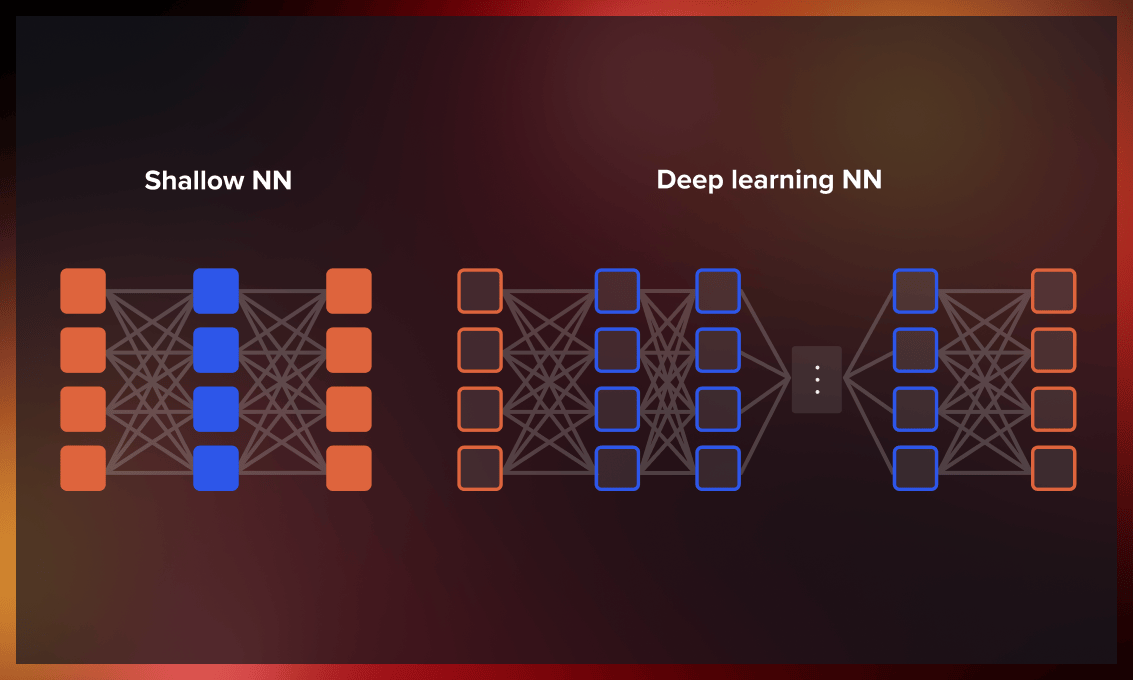
\includegraphics[width=0.8\linewidth]{imagenes/compRNNsWord2Vec.png}
  \caption{Comparativa entre una red neuronal superficial (Word2Vec) y una red neuronal profunda. Fuente: \cite{logunova_word2vec_serokell}.}
  \label{fig:comp_rnns_word2vec}
\end{figure}

El resultado del entrenamiento es la asignación de un vector de cientos de dimensiones a cada palabra del vocabulario. La posición de cada vector en ese espacio no es arbitraria, es decir, palabras empleadas en contextos similares acaban próximas entre sí, mientras que palabras semánticamente distantes se alejan geométricamente.

\begin{figure}[h]
  \centering
  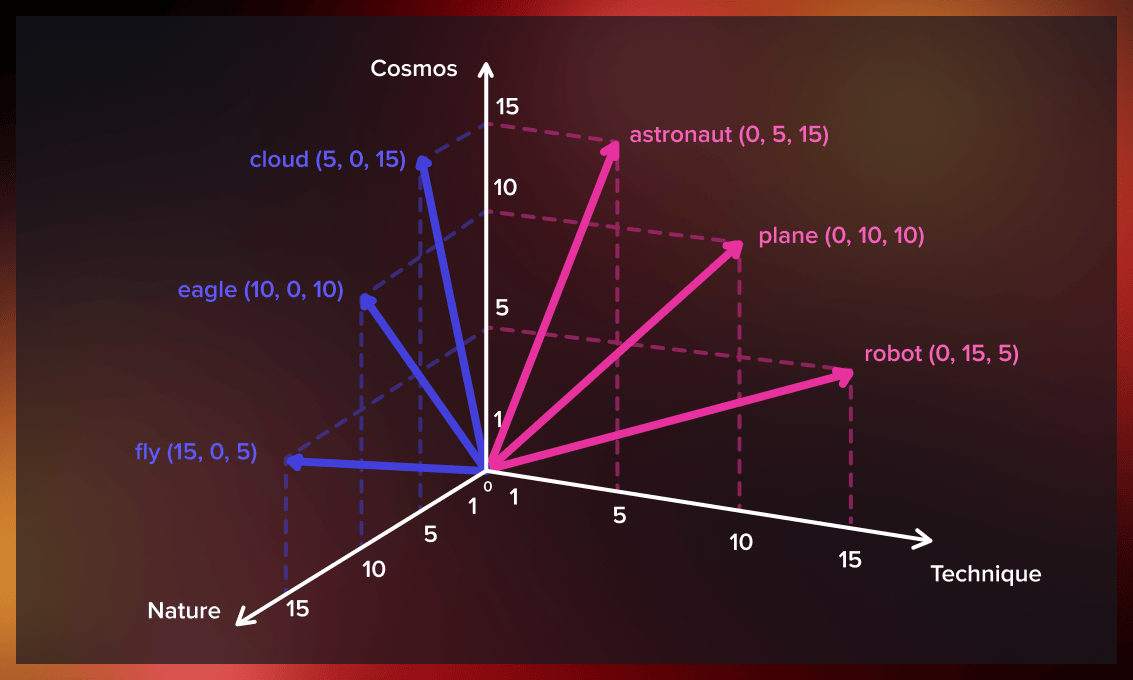
\includegraphics[width=0.8\linewidth]{imagenes/representacionWord2Vec.png}
  \caption{Representación vectorial de palabras en el espacio latente generado por Word2Vec. Fuente: \cite{logunova_word2vec_serokell}.}
  \label{fig:representacion_word2vec}
\end{figure}

Una consecuencia directa de esta estructura es que los vectores admiten operaciones algebraicas con significado semántico. El ejemplo más conocido de esta propiedad es la siguiente analogía entre género y realeza:

\[
  \vec{v}(\text{Rey}) - \vec{v}(\text{Hombre}) + \vec{v}(\text{Mujer}) \approx \vec{v}(\text{Reina})
\]

En esta expresión, al restar al vector de \textit{Rey} la componente que codifica la masculinidad y sumar la que codifica la feminidad, el vector resultante converge hacia la representación de \textit{Reina}. Esta propiedad es inherte a la forma natural del entrenamiento: como \textit{Rey} y \textit{Reina} comparten contextos de realeza pero difieren en los contextos de género, el modelo aprende implícitamente a separar ambas dimensiones dentro del espacio vectorial.

\begin{figure}[h]
  \centering
  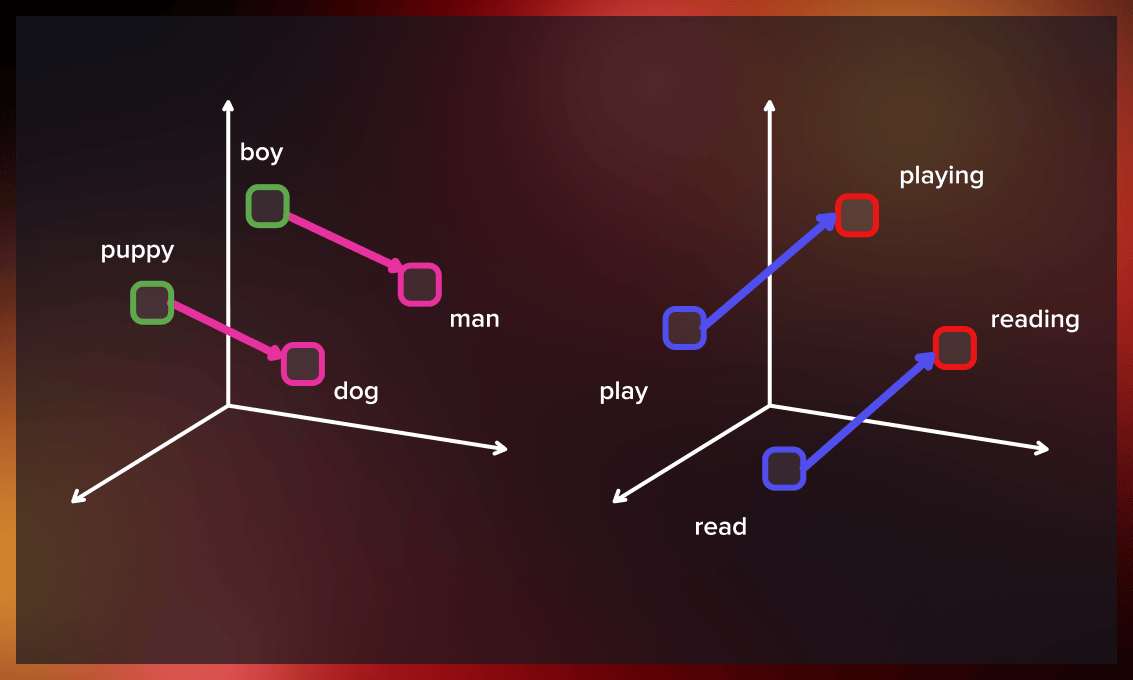
\includegraphics[width=0.8\linewidth]{imagenes/similitudesPalabrasWord2Vec.png}
  \caption{Representación geométrica de las similitudes semánticas entre palabras en el espacio vectorial de Word2Vec. Fuente: \cite{logunova_word2vec_serokell}.}
  \label{fig:similitudes_palabras_word2vec}
\end{figure}

\subsection{Modelos de entrenamiento: \glsentrytext{cbow} y Skip-gram}

Word2Vec ofrece dos variantes arquitectónicas para aprender los vectores de palabras: el modelo \textbf{\glsentrytext{cbow}} y el modelo \textbf{Skip-gram}. Ambos comparten la misma red neuronal superficial como base, pero se diferencian en el aprendizaje, qué se usa como entrada y qué se predice como salida.

En este trabajo se ha optado por implementar el modelo \textbf{Skip-gram}, ya que, como se verá en los capítulos siguientes, sus características lo hacen especialmente adecuado para la adaptación al entorno cuántico propuesto.

\subsubsection{Continuous Bag of Words (\glsentrytext{cbow})}

El modelo \glsentrytext{cbow} toma como entrada las palabras del contexto que rodean a una posición central y predice cuál es la palabra que debería ocupar dicha posición. En otras palabras, dadas las palabras vecinas, el modelo intenta adivinar la palabra central.

\begin{figure}[h]
  \centering
  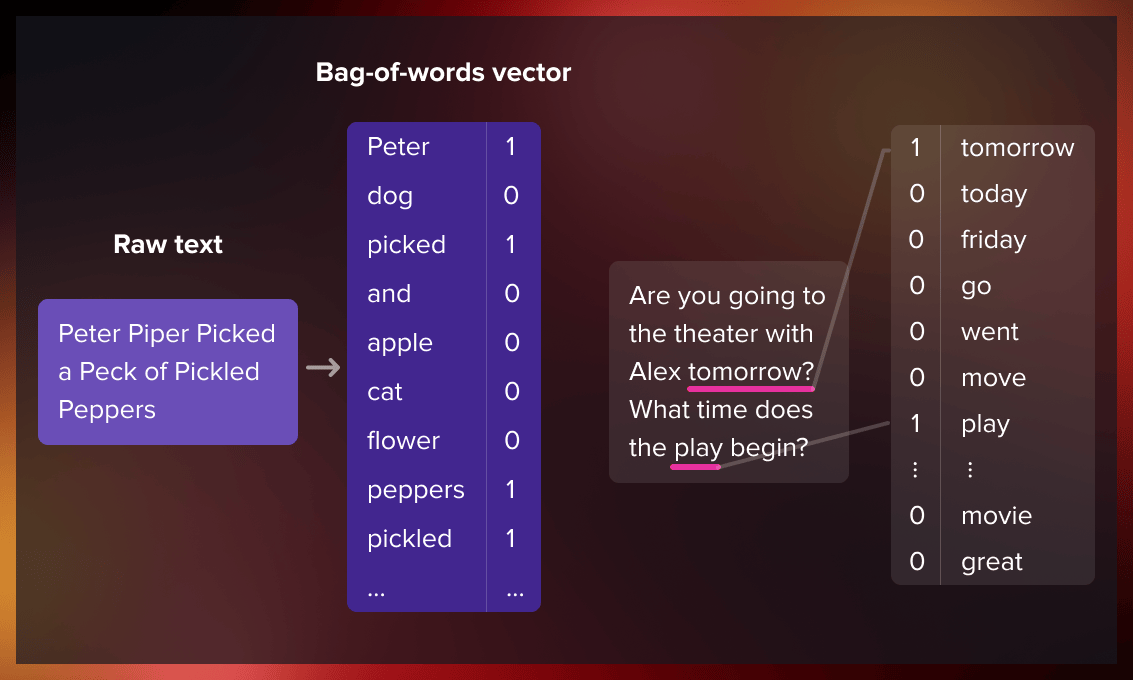
\includegraphics[width=0.8\linewidth]{imagenes/bowExample.png}
  \caption{Ejemplo del funcionamiento del modelo \glsentrytext{cbow}: a partir de las palabras de contexto circundantes se predice la palabra objetivo central. Fuente: \cite{logunova_word2vec_serokell}.}
  \label{fig:cbow_example}
\end{figure}

Este enfoque resulta eficiente cuando el corpus es grande y las palabras frecuentes tienen representaciones ricas. Sin embargo, tiende a promediar la información del contexto, lo que puede penalizar los valores semánticos de palabras menos frecuentes.

\subsubsection{Skip-gram}

Skip-gram es un modelo diseñado para hacer lo opuesto a \glsentrytext{cbow}. En lugar de predecir la palabra central a partir del contexto que tiene en su ventana, toma una única palabra central como entrada e intenta predecir las palabras que aparecen a su alrededor.

El proceso de entrenamiento de esta red neuronal superficial funciona de la siguiente manera: dada la palabra central (la palabra de entrada), se selecciona aleatoriamente una palabra de su contexto inmediato. La red calcula cuál es la probabilidad de que cada palabra del vocabulario sea una palabra "cercana" a la palabra de entrada \cite{mccormick_skipgram_2016}.

Los resultados de estas probabilidades indican cuán probable es que cada término del vocabulario aparezca en las proximidades de la palabra de entrada. Por ejemplo, si la palabra de entrada proporcionada a la red ya entrenada es \textit{reino}, las probabilidades serán considerablemente mayores para palabras como \textit{España} o \textit{Inglaterra} que para términos sin relación semántica como \textit{lápiz} o \textit{mango}.

\subsubsection{Detalles del modelo básico Skip-gram}

Dado que una red neuronal no puede procesar cadenas de texto directamente, cada palabra se representa mediante un \textit{vector one-hot} (una forma de codificación sencilla aunque no la única). Consiste en un vector de tantas componentes como palabras tiene el vocabulario (por ejemplo, 10.000), donde únicamente la posición correspondiente a la palabra de entrada vale 1 y el resto valen 0.

La capa de salida de la red produce también un vector de 10.000 componentes, donde cada valor refleja la probabilidad de que la palabra correspondiente sea una palabra cercana a la entrada. No existe función de activación en la capa oculta, pero la capa de salida aplica \textit{softmax} para normalizar las probabilidades.

\begin{figure}[h]
  \centering
  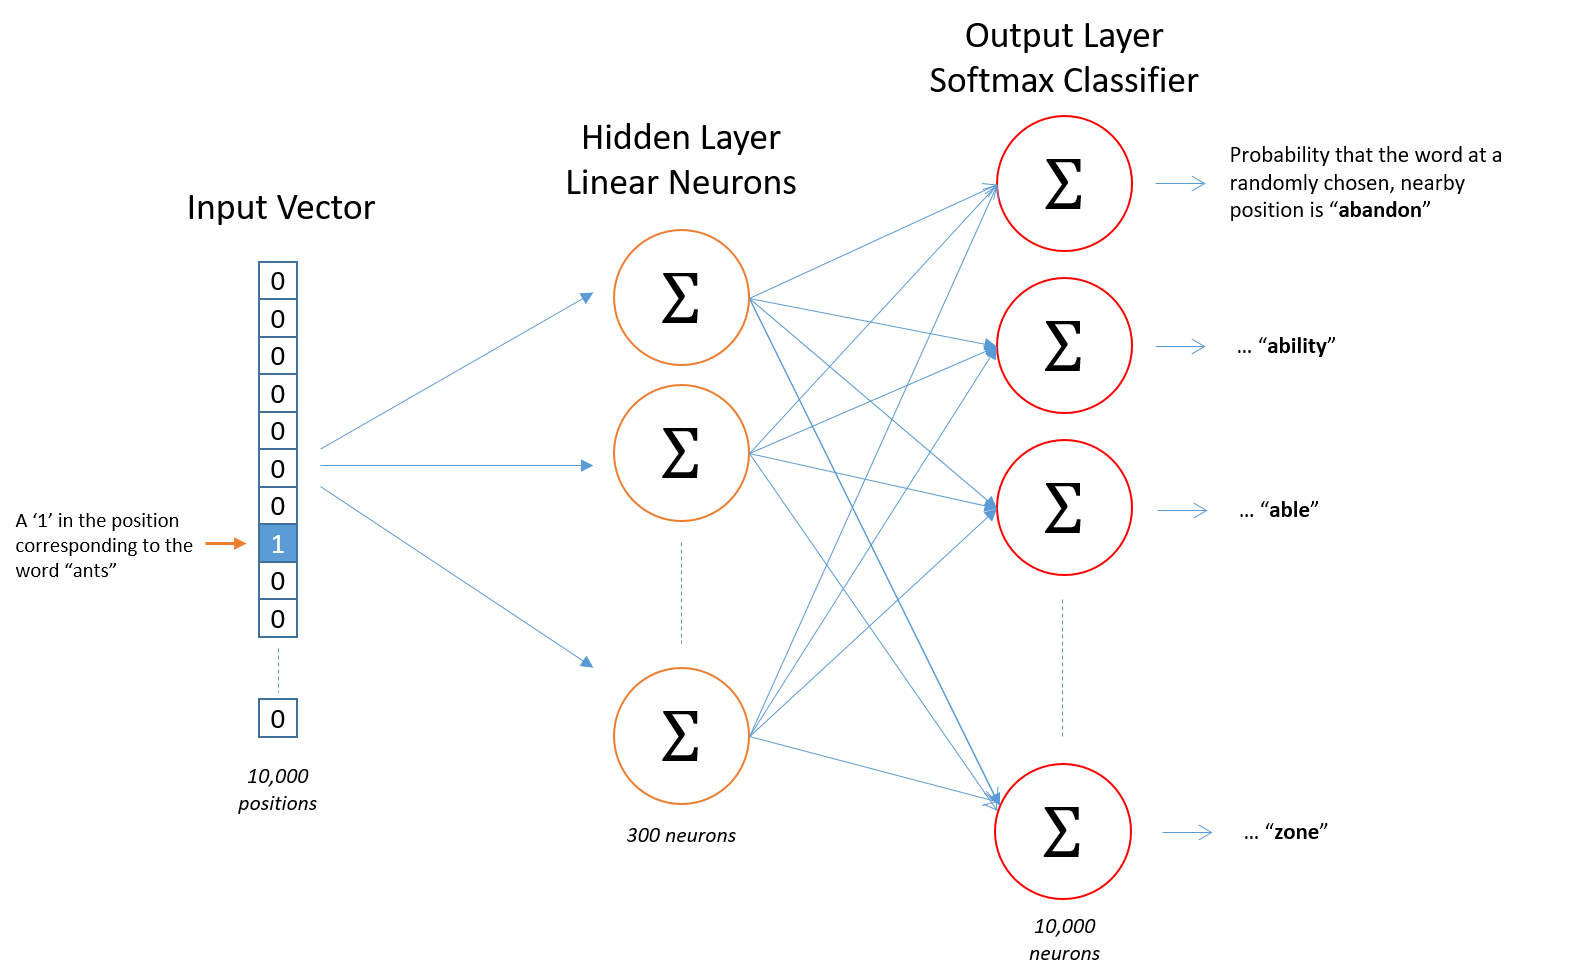
\includegraphics[width=0.7\linewidth]{imagenes/redSkipGram.png}
  \caption{Arquitectura de la red neuronal del modelo Skip-gram. Fuente: \cite{mccormick_skipgram_2016}.}
  \label{fig:red_skip_gram}
\end{figure}

Durante el entrenamiento, tanto la entrada como la salida de la red son vectores \textit{one-hot}. Sin embargo, al evaluar la red con una palabra de entrada, el vector de salida ya no es \textit{one-hot}, sino una distribución de probabilidad sobre todo el vocabulario.

A modo de ejemplo concreto, supóngase que la \textbf{capa oculta} aprende vectores de palabras de 300 dimensiones. En ese caso, los pesos de dicha capa quedan representados por una matriz de $10.000 \times 300$: una fila por cada palabra del vocabulario y una columna por cada neurona oculta. Este es precisamente el tamaño que empleó Google en el trabajo original en el que presentó Word2Vec \cite{google_word2vec_2013}.

Al final, el objetivo de este modelo es aprender la matriz de pesos de la capa oculta. Una vez se tiene esta matriz, la capa de salida es inmediata.

\begin{figure}[h]
  \centering
  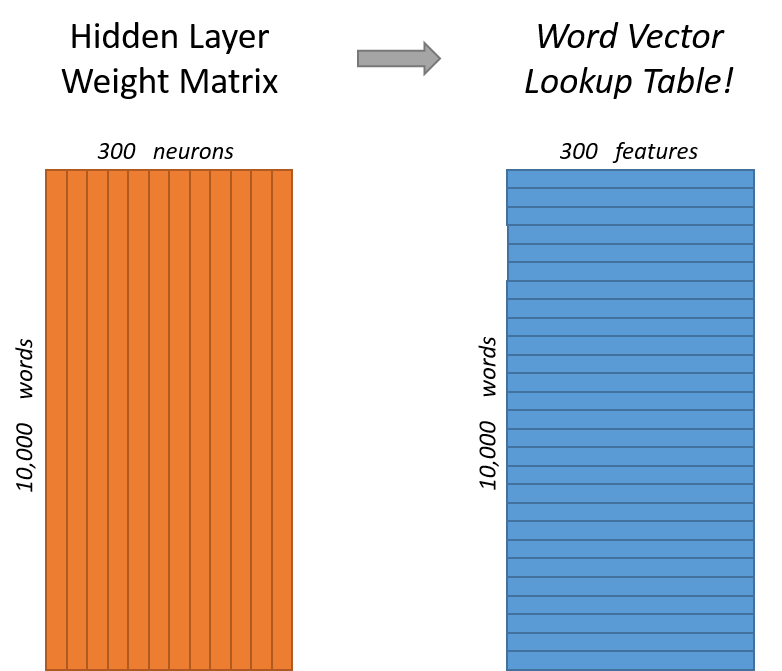
\includegraphics[width=0.6\linewidth]{imagenes/matrizPesosSkipGram.png}
  \caption{Matriz de pesos de la capa oculta del modelo Skip-gram: 10.000 filas (una por palabra del vocabulario) y 300 columnas (una por neurona oculta). Cada fila constituye el vector de representación de su palabra correspondiente. Fuente: \cite{mccormick_skipgram_2016}.}
  \label{fig:matriz_pesos_skip_gram}
\end{figure}

Llegados a este punto, uno puede preguntarse cuál es la utilidad de representar las palabras mediante vectores de todo ceros salvo una única posición con valor $1$. La respuesta reside en la eficiencia, multiplicar un vector \textit{one-hot} de $1 \times 10.000$ por la matriz de $10.000 \times 300$ selecciona de forma inmediata la fila correspondiente a la palabra de entrada, sin necesidad de realizar el producto matricial completo.

\begin{figure}[h]
  \centering
  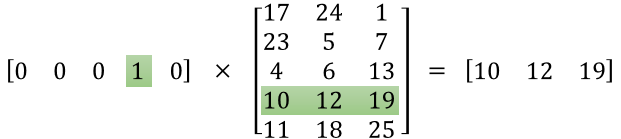
\includegraphics[width=0.7\linewidth]{imagenes/multMatrizOneHot.png}
  \caption{Multiplicación de un vector \textit{one-hot} por la matriz de pesos de la capa oculta, obteniendo directamente el vector de representación de la palabra de entrada. Fuente: \cite{mccormick_skipgram_2016}.}
  \label{fig:mult_matriz_one_hot}
\end{figure}

Con esto se concluye que la capa oculta del modelo actúa en realidad como una tabla \textit{lookup}: la salida de dicha capa es directamente el vector de representación de la palabra de entrada. Así, el vector de $1 \times 300$ resultante se pasa a la \textbf{capa de salida}, que es un clasificador de regresión \textit{softmax}.

Cada neurona de salida produce un valor entre 0 y 1 aplicando la función $\exp(x)$ sobre el producto de su vector de pesos y el vector proveniente de la capa oculta. Para que todos los valores sumen 1 y formen una distribución de probabilidad, cada resultado se divide entre la suma de los valores de las 10.000 neuronas de salida \cite{mccormick_skipgram_2016}.

\begin{figure}[h]
  \centering
  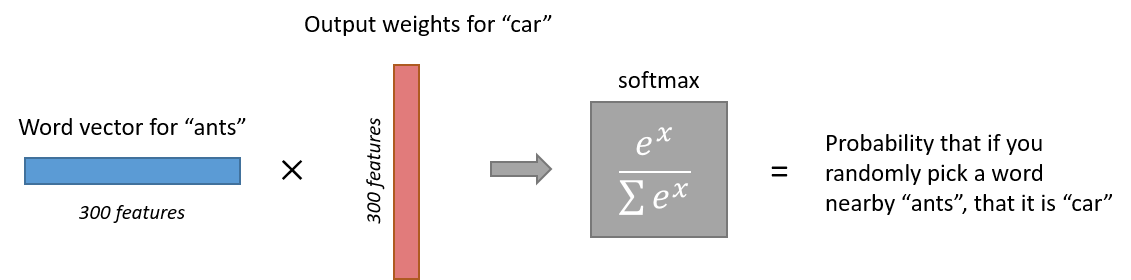
\includegraphics[width=0.9\linewidth]{imagenes/ejemploCapaSalidaSkipGram.png}
  \caption{Cálculo de la salida de la neurona correspondiente a la palabra \textit{car} en la capa \textit{softmax} del modelo Skip-gram. Fuente: \cite{mccormick_skipgram_2016}.}
  \label{fig:ejemplo_capa_salida_skip_gram}
\end{figure}

\section{Función de optimización y pérdida}

\section{Entrenamiento y generación del espacio latente}



\chapter{Implementación Cuántica: Algoritmo QWord2Vec}

En el capítulo anterior se describió en detalle el algoritmo Word2Vec clásico y su variante Skip-gram, que emplea redes neuronales superficiales para aprender representaciones vectoriales de palabras a partir de grandes corpus de texto. En este capítulo se presenta \textit{QWord2Vec}, una adaptación cuántica de dicho modelo propuesta por Ohno \cite{ohno_qword2vec_2025}, cuyo objetivo es explorar si el uso de circuitos cuánticos paramétricos puede ofrecer ventajas en la calidad de las representaciones vectoriales de palabras.

En este capítulo se explorarán la arquitectura del circuito cuántico, la función de coste empleada para su optimización y la estrategia híbrida clásico-cuántica utilizada durante el entrenamiento.

\section{Adaptación del algoritmo al entorno cuántico}

El circuito cuántico de \textit{QWord2Vec} sigue la misma estructura de Word2Vec, compuesta por una parte de \textbf{codificación} y una parte de \textbf{decodificación}. Está formado por puertas de rotación de Pauli (unitarias parametrizadas) y puertas de Pauli-X controladas para introducir entrelazamiento, organizadas en una estructura de capas con profundidad de circuito ajustable. Dado un vector \textit{one-hot} como entrada para una palabra y un vector de salida que representa su contexto \cite{ohno_qword2vec_2025}.

\section{Diseño del Circuito Cuántico Parametrizado}

Como se indicó con anterioridad, la arquitectura de \textit{QWord2Vec} mantiene una estructura análoga a la del algoritmo clásico, dividiéndose en una fase de codificación y otra de decodificación. Esta similitud estructural se ilustra en la Figura \ref{fig:resumen_circuito_qword2vec}.

\begin{figure}[h]
  \centering
  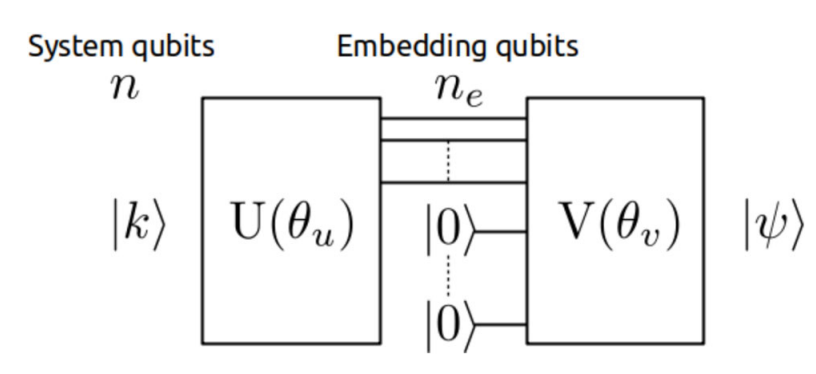
\includegraphics[width=0.9\linewidth]{imagenes/resumenCircuitoQWord2Vec.png}
  \caption{Estructura de QWord2Vec. Fuente: \cite{ohno_qword2vec_2025}.}
  \label{fig:resumen_circuito_qword2vec}
\end{figure}

En la imagen anterior, se aprecia como hay dos matrices parametrizadas, $U(\theta_u)$ y $V(\theta_v)$ junto a una matriz unitaria de entrelazamiento $U(_\text{enta})$. En este sistema, $n$ denota el número total de qubits, mientras que $n_e$ indica el número de qubits destinados específicamente a la representación de los \textit{embeddings}, debiendo cumplirse la restricción $1 \leq n_e \leq n$.

La entrada al circuito viene dada por el estado cuántico $\ket{k}$, el cual representa a una palabra codificada mediante un vector \textit{one-hot}en Word2Vec donde $0 \leq k \leq 2^n - 1$. A partir de este estado inicial, el sistema evoluciona hacia un estado de salida $\ket{\psi}$. Parecido al mapeo directo que realiza Word2Vec, el mapeo que hay entre $\ket{k}$ y $\ket{\psi}$, lo realizan los bloques $U$ y $V$.

Los estados cuánticos de salida resultantes codifican la información correspondiente al contexto de la palabra de entrada, cuya extracción se lleva a cabo realizando mediciones en la base computacional (observable Pauli $Z$).

El modelo $U(\theta_u)$ y $V(\theta_v)$ utilizan las matrices unitarias parametrizadas y las matrices unitarias ($U_\text{enta}$) para proporcionar el entrelazamiento cuántico de la siguiente manera:

\[
  U(\theta) = \prod_{l=1}^{L}
  U_{\text{enta}}\,
  R_Z\!\left(\theta_z^{L-l+1}\right)^{\otimes n}
  R_Y\!\left(\theta_y^{L-l+1}\right)^{\otimes n}
  R_X\!\left(\theta_x^{L-l+1}\right)^{\otimes n}
\]

donde $L$ representa la longitud del circuito cuántico. Por simplicidad, se asumirá que tanto $U(\theta_u)$ como $V(\theta_v)$ poseen la misma profundidad, a menos que se indique explícitamente lo contrario.

Para implementar $U_\text{enta}$, se ha usado puertas controladas Pauli $X$ (CNOT), siguiendo una configuración de circuito por bloques \cite{sim2019expressibility}. Esta disposición favorece notablemente la expresividad del circuito y maximiza su capacidad para generar entrelazamiento. La Figura \ref{fig:qword2vec_circuit} muestra visualmente la estructura del circuito resultante al combinar las rotaciones de Pauli con el bloque de entrelazamiento descrito.

\newpage
\begin{figure}[h]
  \centering
  
\includegraphics[width=1.0\linewidth]{imagenes/qword2vec_circuit.png}
  \caption{Circuito cuántico parametrizado de QWord2Vec con puertas de rotación de Pauli ($R_X$, $R_Y$, $R_Z$) y entrelazamiento con configuración por bloques mediante puertas CNOT.}
  \label{fig:qword2vec_circuit}
\end{figure}

El uso combinado de las tres puertas de rotación ($R_X, R_Y, R_Z$) permite que los estados cuánticos que representan a las distintas palabras alcancen una mayor dispersión en el espacio de Hilbert, superando las limitaciones de representatividad que se obtendrían empleando una sola matriz de rotación, tal y como se observa en la Figura \ref{fig:esferas_bloch_rotaciones_pauli}.

\begin{figure}[h]
  \centering
  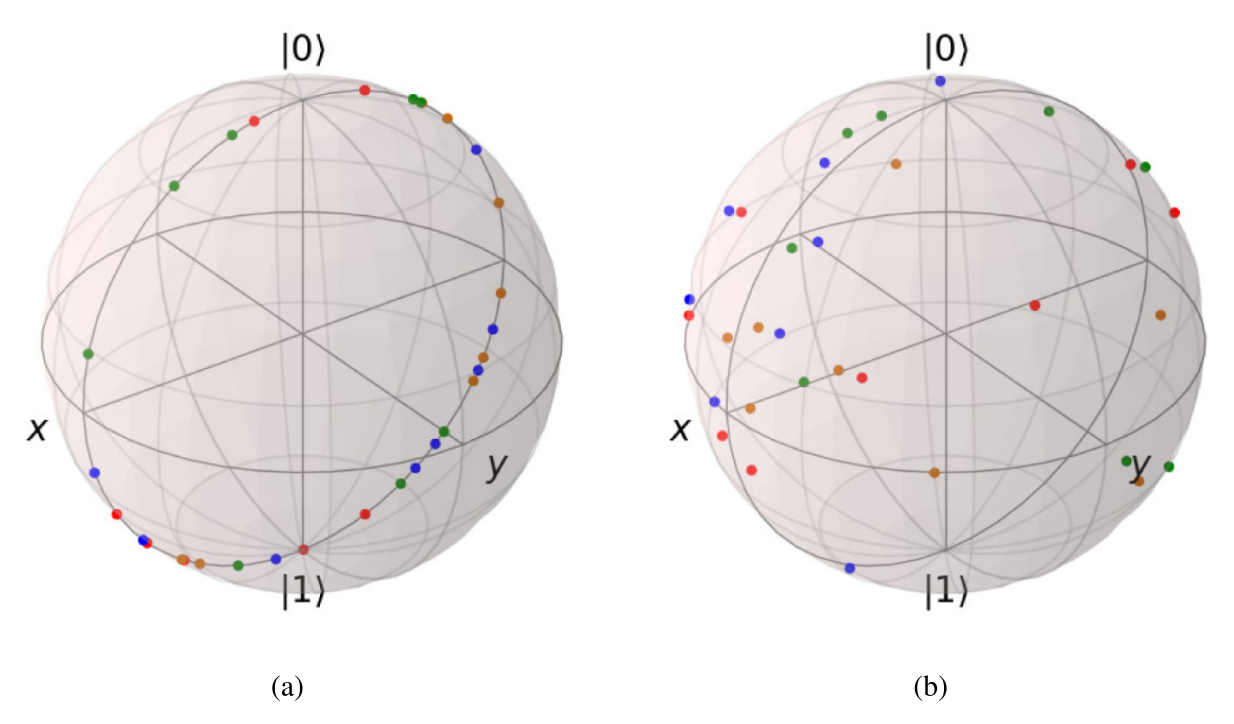
\includegraphics[width=0.9\linewidth]{imagenes/esferaBlochRotacionesPauli.png}
  \caption{Representación de las palabras sobre la esfera de Bloch según las puertas de rotación empleadas en $U(\theta_u)$: (a) usando únicamente $R_Y$, y (b) usando $R_X$, $R_Y$ y $R_Z$ combinadas. Los puntos coloreados corresponden a las palabras y el número total de puntos es 32. El uso de las tres puertas de rotación de Pauli permite una mayor dispersión de las representaciones a lo largo del espacio de Hilbert. Fuente: \cite{ohno_qword2vec_2025}.}
  \label{fig:esferas_bloch_rotaciones_pauli}
\end{figure}

\section{Definición de la función de evaluación y pérdida usadas}

\subsection{Evaluación de los datos de embeddings}

Para evaluar la calidad de los \textit{embeddings} generados por QWord2Vec, se emplea el coeficiente de correlación de Pearson, calculado a partir de las distancias entre los vectores producidos por ambos modelos, Word2Vec y QWord2Vec.

Una vez completado el entrenamiento, se realiza una medición sobre los qubits destinados a los \textit{embeddings}, obteniendo así los vectores clásicos correspondientes a cada palabra. A partir de estos vectores, se construye un \textit{vector distancia}, cuyas componentes son las distancias euclídeas entre los vectores de \textit{embeddings} de todas las palabras del vocabulario. Este proceso se aplica tanto al modelo clásico como al cuántico, tomando el vector distancia de Word2Vec como referencia de comparación (\textit{ground truth}).

El motivo por el que no se utiliza únicamente la entropía cruzada como métrica de evaluación reside en que los circuitos cuánticos con un elevado número de parámetros tienden a reducir su valor. Por ello, se añade el coeficiente de correlación de Pearson sobre los vectores distancia ya que constituye una métrica más adecuada y robusta para valorar la capacidad del modelo. En la siguiente subsección se describe en detalle la función de pérdida empleada durante el entrenamiento del circuito.

\subsection{Función de pérdida}

La función de pérdida usada, además de tener el componente de la pérdida de entropía cruzada, se le añade un término junto al coeficiente de correlación de Pearson. Por lo que la función de pérdida queda de la siguiente manera:

\[
  \text{Loss} := \text{CrossEntropyLoss} - C \cdot \text{CorrelationCoefficient}(\textit{EmbeddingData}, \textit{ReferencesDistances}),
\]

Donde $C > 0$ es un parámetro de balanceo. $\text{CorrelationCoefficient}(\textit{EmbeddingData}, \textit{ReferencesDistances})$ se refiere al coeficiente de correlación entre el vector distancia de los datos de embeddings (\textit{EmbeddingData}) en QWord2Vec el cual se actualiza en cada iteración mientras que \textit{ReferencesDistances}, se refiere al vector de distancias referencias en este caso el obtenido de Word2Vec.




\section{Estrategia de optimización híbrida (Clásica-Cuántica)}



\chapter{Experimentación y Análisis de Resultados}
\label{chap:experimentacion}

Una vez descritos los fundamentos teóricos de Word2Vec y QWord2Vec, este capítulo recoge el proceso de experimentación llevado a cabo para comparar ambos modelos. Se han desarrollado las implementaciones de ambos algoritmos en el lenguaje de programación \textit{Python}.

Para el modelo clásico, se ha empleado la implementación disponible en la librería \textit{Gensim}, que incluye tanto la arquitectura del modelo como la función de optimización Negative Sampling, desarrollada siguiendo las especificaciones originales de Google. Por su parte, la versión cuántica ha sido implementada utilizando la librería \textit{Qiskit}, que proporciona las herramientas necesarias para la construcción del circuito parametrizado, la aplicación del optimizador descrito en el capítulo anterior, así como utilidades para la medición y transpilación del circuito.

El objetivo principal de esta experimentación es evaluar si los \textit{embeddings} generados por QWord2Vec son capaces de preservar relaciones semánticas entre palabras de forma comparable a los producidos por Word2Vec. Para ello, se ha seguido una metodología sistemática que abarca desde la preparación del corpus y la configuración de los hiperparámetros, hasta el análisis de la función de pérdida durante el entrenamiento y la evaluación de la calidad de los \textit{embeddings} mediante el coeficiente de correlación de Pearson. Asimismo, se incluye un análisis comparativo de los tiempos de ejecución de ambos modelos, dado que el coste computacional es uno de los factores críticos en el contexto de la computación cuántica simulada.

\section{Metodología experimental}

Esta sección describe los pasos previos necesarios para llevar a cabo la experimentación. En primer lugar, se presenta el corpus empleado para el entrenamiento de ambos modelos, junto con el proceso de preprocesamiento aplicado en cada caso. A continuación, se detallan las herramientas y el entorno de ejecución utilizados, aspecto especialmente relevante en el caso de QWord2Vec, dado que la simulación clásica de circuitos cuánticos impone restricciones significativas sobre el tamaño del experimento realizable.

\subsection{Dataset y preprocesamiento}

Como se comentó anteriormente, la simulación clásica de circuitos cuánticos impone restricciones severas sobre el tamaño del experimento. A diferencia de Word2Vec clásico, que habitualmente se entrena con corpus de millones de frases y vocabularios de cientos de miles de palabras, el coste computacional de simular un circuito cuántico crece exponencialmente con el número de qubits, lo que hace inviable trabajar con corpus de gran escala en un entorno de computación personal que es con el que se ha trabajado.

Por este motivo, se ha adoptado el mismo corpus empleado en el trabajo de referencia \cite{ohno_qword2vec_2025}, el cual fue tomado originalmente de una fuente web la cual ofrecía corpus pequeños para realizar evaluaciones de modelos de este estilo, solo que actualmente no está disponible la página web. El corpus consta de 13 frases en inglés con un vocabulario de 13 palabras únicas. Las frases utilizadas son las siguientes:

\begin{quote}
  \ttfamily
  i like dog \quad i like cat \quad i like animal \quad dog cat animal \\
  apple cat dog like \quad dog fish milk like \quad dog cat eyes like \\
  i like apple \quad apple i hate \quad apple i movie \\
  book music like \quad cat dog hate \quad cat dog like
\end{quote}

Las frases tienen una longitud de entre 3 y 4 palabras, lo que condiciona el tamaño de la ventana de contexto haciendo que sea pequeña. Desde el punto de vista de la distribución léxica, el corpus presenta un desequilibrio: las cuatro palabras más frecuentes (\textit{like}, \textit{dog}, \textit{cat} e \textit{i}) concentran el 67\% de los tokens totales, mientras que seis palabras del vocabulario aparecen una única vez. Este desequilibrio puede introducir distorsiones en las relaciones semánticas aprendidas por el modelo, y es una limitación que se asume de forma consciente.

No obstante, el uso de este corpus está justificado por tres razones. En primer lugar, permite reproducir directamente las condiciones experimentales del paper de referencia, facilitando la comparación de resultados durante el desarrollo e implementación de variaciones que se han realizado. En segundo lugar, el objetivo del estudio no es obtener un modelo de procesamiento del lenguaje natural de calidad, sino evaluar si QWord2Vec es capaz de preservar las relaciones semánticas que aprende Word2Vec. Para este fin, un corpus pequeño y controlado es suficiente. En tercer lugar, el tamaño reducido del vocabulario permite inspeccionar e interpretar los \textit{embeddings} obtenidos de forma directa, verificando manualmente que las relaciones semánticas resultantes son coherentes con el contenido del corpus.

En cuanto al preprocesamiento, no se ha realizado nada ya que el corpus viene preprocesado con sus palabras separadas por un espacio tal y como se espera sin necesidad de haber tenido que eliminar algún signo de puntuación o bien convertir todo a minúscula.

\subsection{Entorno de ejecución y herramientas}

Todos los experimentos se han llevado a cabo sobre un ordenador personal con sistema operativo Ubuntu, cuya compatibilidad con las librerías empleadas y su integración con el hardware disponible lo hacen especialmente adecuado para este tipo de desarrollo. Las características del hardware relevantes para el rendimiento son las siguientes:

\begin{itemize}
  \item \textbf{Procesador}: Intel Core i7-13700F (30\,MB de caché, frecuencia máxima superior a 5,2\,GHz).
  \item \textbf{Memoria RAM}: 32\,GB DDR4 a 3600\,MHz.
  \item \textbf{Tarjeta gráfica}: MSI GeForce RTX 4070 con 12\,GB de memoria GDDR6X.
\end{itemize}

En cuanto al software, las librerías principales utilizadas en el desarrollo son:

\begin{itemize}
  \item \textbf{Python} 3.10.12: lenguaje de programación base del proyecto.
  \item \textbf{Gensim} 4.4.0: empleada para la implementación del modelo Word2Vec clásico.
  \item \textbf{Qiskit} 1.4.5: utilizada para la construcción y ejecución del circuito cuántico parametrizado.
  \item \textbf{Qiskit Aer} 0.17.2: backend de simulación cuántica sobre hardware clásico.
\end{itemize}

Respecto a la elección del simulador cuántico, \textit{Qiskit} ofrece tres opciones: \textit{AerSimulator}, \textit{StatevectorSimulator} y \textit{QasmSimulator}. Los dos últimos se encuentran en proceso de deprecación, dado que \textit{AerSimulator} los unifica y supera en capacidades siendo el que más soporte y desarrollo recibe. Por este motivo, se ha optado por \textit{AerSimulator} como backend de simulación para la ejecución de QWord2Vec.

\section{Configuración de hiperparámetros}

Tanto el modelo clásico como el cuántico presentan una serie de hiperparámetros que deben ajustarse para obtener el mejor rendimiento posible, como ocurre en cualquier problema de \gls{ml}. Para su configuración se ha empleado la técnica de búsqueda exhaustiva \textit{Grid Search}, implementada manualmente en ambos casos al no disponer de una implementación genérica compatible con los modelos utilizados.

La estrategia seguida ha consistido en identificar, a partir de la literatura y de experiencias previas en problemas similares que han comentado distintas personas en foros, un conjunto de valores de referencia para cada hiperparámetro. A partir de estos valores, se han definido rangos de búsqueda que incluyen el valor de referencia junto con variaciones por encima y por debajo, con el objetivo de ajustar cada parámetro al corpus y al problema concreto. Dado que ambos modelos emplean funciones de pérdida y algoritmos de optimización distintos, cada uno dispone de su propio conjunto de hiperparámetros a explorar.

\subsection{Hiperparámetros de Word2Vec}

Los hiperparámetros de Word2Vec pueden agruparse en tres categorías según el componente del modelo al que pertenecen: los propios de la arquitectura Skip-Gram, los relacionados con Negative Sampling y el correspondiente al optimizador.

En cuanto a los hiperparámetros de \textbf{Skip-Gram}, los dos parámetros ajustados son \textit{vector\_size} y \textit{window}. El primero determina la dimensionalidad de los vectores de \textit{embedding}, es decir, el número de características con el que se representa cada palabra. Su elección depende del tamaño del vocabulario, la riqueza semántica del corpus y los recursos computacionales disponibles. Dado que el vocabulario es de únicamente 13 palabras, no se requiere una representación de alta dimensionalidad para capturar las relaciones semánticas presentes. Por ello, se exploraron valores en el rango $\{2, 3, 4\}$. El valor seleccionado por el \textit{Grid Search} fue $\text{vector\_size} = 2$, lo cual resulta coherente con el reducido tamaño del vocabulario y presenta la ventaja adicional de permitir visualizar directamente los \textit{embeddings} en el plano y realizar una validación manual sin necesidad de aplicar técnicas de reducción de dimensionalidad como PCA.

El segundo parámetro, \textit{window}, define la distancia máxima entre la palabra central y las palabras de contexto consideradas durante el entrenamiento, tal y como se ilustra en la Figura \ref{fig:window_ilustracion}. Los valores explorados fueron $\{1, 2, 3\}$, teniendo en cuenta que las frases del corpus tienen entre 3 y 4 palabras: con una ventana de tamaño 2, la palabra central puede relacionarse con todas las demás en una frase de 4 palabras, mientras que con tamaño 1, solo se considera la palabra adyacente. El valor seleccionado fue $\text{window} = 1$, lo que implica que el modelo aprende exclusivamente a partir de pares de palabras contiguas, una restricción adecuada dada la brevedad de las frases del corpus.

\begin{figure}[h]
  \centering
  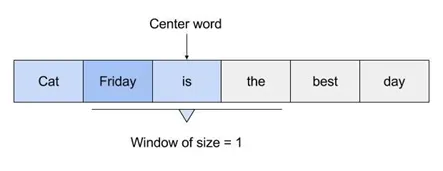
\includegraphics[width=0.7\linewidth]{imagenes/windowIlustration.png}
  \caption{Ilustración del parámetro \textit{window} en Skip-Gram: distancia máxima desde la palabra central hasta las palabras de contexto consideradas. Fuente: \url{https://medium.com/@zafaralibagh6/a-simple-word2vec-tutorial-61e64e38a6a1}.}
  \label{fig:window_ilustracion}
\end{figure}

Respecto a los hiperparámetros de \textbf{Negative Sampling}, los parámetros explorados son \textit{negative} y \textit{ns\_exponent}. El primero indica el número de muestras negativas que se generan por cada par positivo durante el entrenamiento. El paper original que publicó Google, recomendó valores entre 5 y 20 (siendo 20 para corpus de gran escala). Dado que el corpus empleado cuenta únicamente con 13 palabras únicas, se optó por explorar valores en el rango $\{2, 3, 5, 6\}$, descartando valores superiores a la mitad del vocabulario para evitar que Negative Sampling degenerase en un comportamiento equivalente al softmax completo sobre todo el vocabulario, además de tener en consideración la recomendación del paper de Google. El valor seleccionado fue $\text{negative} = 5$, coincidiendo con el mínimo recomendado en el paper original.

El parámetro \textit{ns\_exponent} controla la distribución de probabilidad con la que se seleccionan las palabras negativas. Un valor de 1 desfavorece a las palabras poco frecuentes respecto a una distribución puramente proporcional a las frecuencias, mientras que un valor de 0,0 trata todas las palabras con igual probabilidad. El paper original de Word2Vec estableció 0,75 como valor fijo, sin embargo, un estudio posterior \cite{caselles_word2vec_hyperparameters_2018} argumentó que este parámetro debería adaptarse al problema concreto. Dado el notable desequilibrio léxico del corpus utilizado, se exploraron los valores $\{0{,}0,\ 0{,}3,\ 0{,}75\}$. El valor seleccionado fue $\text{ns\_exponent} = 0{,}0$, lo que implica que todas las palabras tienen igual probabilidad de ser seleccionadas como muestras negativas, compensando en parte el desequilibrio de frecuencias del corpus.

Por último, el hiperparámetro relacionado con el \textbf{optimizador} es \textit{alpha}, que establece la tasa de aprendizaje inicial del modelo. \textit{Gensim} gestiona internamente la evolución de esta tasa a lo largo del entrenamiento, permitiendo únicamente fijar su valor inicial. La búsqueda de este parámetro se realizó en dos fases iterativas. En una primera exploración se consideró el rango $\{0{,}1,\ 0{,}15,\ 0{,}175,\ 0{,}2\}$, con el objetivo de comprobar si valores pequeños eran suficientes para la convergencia. El valor seleccionado en esta fase fue $0{,}2$, el límite superior del rango, lo que indicó que el modelo requería tasas de aprendizaje más elevadas. A partir de este resultado, se acotó el rango de búsqueda hacia valores superiores, explorando $\{0{,}2,\ 0{,}25,\ 0{,}275,\ 0{,}3\}$. En esta segunda fase el valor seleccionado fue $\text{alpha} = 0{,}25$, situándose en el interior del rango y confirmando que la convergencia óptima se alcanza con tasas de aprendizaje relativamente elevadas.


\subsection{Hiperparámetros de QWord2Vec}

En cuanto a los hiperparámetros de la parte cuántica, se puede dividir en 3 bloques principales que son: Hiperparámetros del circuito, hiperparámetros relacionados con \gls{qng} y los hiperparámetros relacionados con \gls{spsa}. Estos 2 últimos, en la clase utilizada la cual tiene el algoritmo \gls{qn-spsa} implementado, contiene los hiperparámetros relacionados a \gls{qng} y los relacionados a \gls{spsa} para juntarlos en el algoritmo que los engloba.

En cuanto a los hiperparámetros del circuito, solo se puede tener en cuenta el número de iteraciones que realiza así como el número de muestras que toma en una simulación. Para el primer hiperparámetro, se ha tenido en cuenta que los circuitos variacionales cuánticos suelen necesitar muchas épocas para converger. El paper principal en el que se ha basado para implementar este circuito cuántico \cite{ohno_qword2vec_2025}, utilizó para su circuito un máximo de 30.000 épocas (utilizando otra función de optimización menos eficiente que la que se ha propuesto aquí). Por lo que teniendo en cuenta el número de épocas tan grande pero que también la función de optimización \gls{qn-spsa} está diseñada para que converga con pocas épocas, decidí utilizar 1500 iteraciones como máximo. En cuanto al número de muestras obtenidas en cada simulación, seleccioné una gran cantidad para tener una distribución de valores más limpia y exigente, siendo así los resultados lo más honesto posibles evitando que haya mucha varianza estadística, por ello utilicé 1024 shots por cada simulación. Otro hiperparámetro a configurar, fue el valor \textit{A\_{th}} que se utiliza en la fórmula del cálculo heurístico de número de capas, este parámetro viene a indicar cuál es el límite superior de datos de entrenamiento que se está dispuesto a perder. Para establecer este valor, se ha tenido en cuenta que en el paper el cual indicaba la heurística para calcular la longitud del circuito, indicaba que los mejores parámetros de \textit{A\_{th}} que le funcionó, estaban entre 0.01 y 0.05. Por ello en el gird search primero se probó con valores muy dispares de 0.01, 0.03 y 0.05 y viendo que se quedó con el 0.03 luego se probó valores algo superiores e inferiores a 0.03 encontrando así que el mejor Ath posible para el corpus que se tiene y el resto de hiperparámetros calculados ha sido 0.21.

Para los hiperparámetros de SPSA, en concreto los que gestiona cómo va decayendo la tasa de aprendizaje y la perturbación, se ha utilizado las fórmulas que indica el autor en su paper original de este algoritmo \cite{spall_spsa_1998}. De estas fórmulas, hay 4 valores posibles a ajustar, que son: los 2 coeficientes de cuanto decaimiento tienen los valores de la tasa de aprendizaje y de perturbación a lo largo de las épocas y luego los otros 2 coeficientes iniciales del leraning rate y perturbación. Pues bien, de estos 4 posibles valores, solo se han fine tuneado los 2 últimos. Esto se ha decidido así porque como bien indica en el paper, los valores de decaimiento que propone ya han sido probados matemáticamente y empíricamente por lo que son los valores recomendables a utilizar mientras que los valores de la tasa de aprendizaje inicial así como de la perturbación son valores que se tienen que ajustar a cada tipo de problema. Teniendo eso en cuenta, se probó con valores bajos de learning rates y de perturbaciones sabiendo que se aplicaba un educated guess al inicio. Un educated guess significa que en vez de elegir valores aleatorios de pesos, se prueba de manera aleatoria durante un cierto número de iteraciones de y se queda con aquellos pesos que hayan dado mejores resultados en las simulaciones. En este caso el educated guess ha sido de 10 iteraciones por cada parámetro. Teniendo en cuenta esta pequeña técnica aplicada para mejorar los pesos iniciales, fue uno de los motivos principales por los que no se quiso usar un learning rate alto, es decir, ya se tendrían unos hiperparámetros que podrían ir en buena dirección. <cuando corrigas esto Claude, méteme algún argumento mejor o algo de por qué usar valores pequeños para los hiperaprámetros de inicio de learning rate y de perturbación>

Además se decidió establecer el parámetro \textit{blocking} a true para que así el optimizador solo aceptara mejoras de un valor de pérdida no más grande que el anterior actualizado añadido con una tolerancia.

El resto de parámetros a configurar, ha sido todo lo relacionado con el \gls{qng}, al principio he buscado en la literatura clásica que venía explicada \cite{duan_qnspsa_pennylane_2022} cuáles eran los hiperparámetros que se debían de ajustar. De ahí se siguió las recomendaciones de configurar el tensor métrico de Fubiny-Study como la matriz identidad en $g^{(0)}$. También se tomó en consideración buscar el mejor valor del hiperparámetro del coeficiente de regularización, así cuando se aplicara el valor del tensor métrico de Fubiny-Study cerca de un mínimo, no se desvaneciera dicho tensor. De este hiperparámetro se tuvo en cuenta las consideraciones de no tomar un valor muy alto ya que eliminaría toda la información del tensor mético de Fubiny-Study pero un valor muy bajo haría que se desvaneciera en el límite. Además para validar si sería necesario utilizar esta función de optimización ya que es muy compleja además de que tiene mucha potencia, se ha decidido establecer otro hiperparámetro que es el \textit{Hessian Delay}, este hiperparámetro controla cuando se debe de aplicar el tensor métrico de Fubiny-Study. Esto se ha decidido establecer ya que al principio con mucho ruido puede hacer que no se comporte bien del todo. Además se ha establecido otro hiperparámetro que es el resampling. Esto indica cuántas veces se tiene que ejecutar el cálculo del tensor métrico de Fubiny-Study y hacer una media de los valores obtenidos. Se ha puesto un resampling bajo ya que este introduce una mayor sobrecarga a lo dificultoso que es de ejecutar el algoritmo de por si. Se ha establecido este hiperparámetro con el objetivo de ver si es necesaria tanta complejidad en la función de optimización para este problema, o bien utilizando solo el SPSA al igual que hace el paper original pero con unos mejores hiperparámetros, daba mejores resultados. Otro hiperparámetro que ha habido que establecer es la fidelidad, para calcular este tensor a nivel práctico se tiene que hacer sobre el circuito que se quiere optimizar. En este caso al ser un corpus de 13 palabras, se tienen 13 circuitos distintos ya que cada uno tiene su codificación de manera independiente en el espacio de Hilbert. Por lo que para no calcular siempre el tensor métrico de Fubiny-Study sobre el mismo circuito, se ha ido rotando de manera uniforme para que calculara el valor con distintos circuitos y así evitar que solo afectara a una palabra perjudicando a todas las demas palabras utilizadas.

\section{Entrenamiento}

En esta sección se describe el proceso de entrenamiento seguido para cada modelo. Dado que Word2Vec y QWord2Vec emplean funciones de pérdida y algoritmos de optimización distintos, el análisis de cada uno se presenta de forma independiente.

\subsection{Word2Vec}

El proceso de entrenamiento de Word2Vec se basa en la función de pérdida de Negative Sampling como se explicó con anterioridad. Sin embargo, minimizar esta función auxiliar no garantiza directamente una buena calidad semántica de los \textit{embeddings}. Por ello, se ha incorporado una métrica de evaluación adicional basada en el algoritmo \textit{K-Means}, que permite cuantificar de forma directa la coherencia semántica de los vectores obtenidos.

El rol de cada componente es el siguiente. \textbf{Train loss} actúa como función de optimización, proporcionando la señal con la que el optimizador actualiza los parámetros en cada iteración. El \textbf{K-Means accuracy} constituye la métrica de calidad real de los \textit{embeddings} y es la que determina el criterio de parada. Esta distinción es importante, usar el loss como criterio de \textit{Early Stopping} podría interrumpir el entrenamiento en un punto subóptimo desde el punto de vista semántico, ya que el loss de Negative Sampling puede seguir oscilando incluso cuando los \textit{embeddings} han convergido a su mejor configuración.

Para calcular la precisión de \textit{K-Means}, es necesario disponer de un agrupamiento (también conocido como clusters) de referencia (\textit{ground truth}) de las palabras del vocabulario. Dicho agrupamiento fue generado mediante el modelo de lenguaje Gemini 3.0 Pro a partir del corpus, con la restricción de que los grupos fueran lo más equilibrados posible y sin poder aparecer la misma palabra en distintos grupos. El resultado fue posteriormente validado manualmente, obteniéndose los siguientes cuatro clústeres:

\begin{itemize}
  \item \textbf{animal}: \textit{dog, cat, animal, eyes}
  \item \textbf{food}: \textit{apple, fish, milk}
  \item \textbf{culture}: \textit{book, music, movie}
  \item \textbf{sentiment}: \textit{i, like, hate}
\end{itemize}

Dado que \textit{K-Means} asigna etiquetas arbitrarias a los clústeres, la precisión se calcula mediante el algoritmo húngaro, que encuentra la correspondencia óptima entre los clústeres predichos y los de referencia antes de evaluar el porcentaje de palabras correctamente asignadas.

Esta evaluación no se realiza en cada época, sino cada 200 épocas de entrenamiento. Esta frecuencia permite que el modelo evolucione suficientemente entre comprobaciones, manteniendo un equilibrio entre la sensibilidad de la métrica y la carga computacional adicional que supone ejecutar \textit{K-Means} sobre los \textit{embeddings} actuales.

La técnica de \textit{Early Stopping} monitoriza el K-Means accuracy en cada comprobación y detiene el entrenamiento si no se supera el mejor valor previo en al menos un delta mínimo de 0,01 durante 5 comprobaciones consecutivas (paciencia = 5). En ese punto se recupera los pesos de los parámetros correspondiente al mejor accuracy registrado, reduciendo el riesgo de sobreajuste y garantizando que el modelo devuelto es el que mejor agrupa semánticamente las palabras.

Respecto a la partición de los datos, el entrenamiento se ha realizado con el 100\% del corpus, sin reservar un conjunto de validación o prueba. Esta decisión fue tomada ya que uno de los objetivos del experimento de la versión clásica no es evaluar la capacidad de generalización del modelo a palabras nuevas, sino obtener \textit{embeddings} de referencia para todas las palabras del vocabulario. Dado que Word2Vec solo genera un vector para una palabra si la ha observado durante el entrenamiento, excluir un subconjunto de frases implicaría que algunas palabras del vocabulario carecerían de embedding, dificultando la comparación con QWord2Vec, que requiere los vectores de referencia de todo el corpus.

En cuanto al flujo de entrenamiento, las frases del corpus se reordenan aleatoriamente antes del entrenamiento para evitar que el modelo aprenda varias frases consecutivas cuyos valores están definidos en el mismo clúster, favoreciendo una exploración más amplia del espacio de parámetros. Se utiliza una semilla fija (valor 42) para garantizar la reproducibilidad de los resultados. El modelo se entrena desde cero utilizando los mejores hiperparámetros encontrados en el \textit{Grid Search}. Una vez finalizado el entrenamiento, los \textit{embeddings} de la mejor época encontrada, se exportan a un fichero de texto plano para su uso como referencia de comparación en la implementación cuántica.

La evolución del K-Means accuracy y del train loss delta a lo largo del entrenamiento se puede observar en la Figura \ref{fig:loss_curves_word2vec}.

\begin{figure}[h]
  \centering
  
\includegraphics[width=0.85\linewidth]{imagenes/lossCurvesWord2Vec.png}
  \caption{Evolución del K-Means accuracy (eje izquierdo, naranja) y del train loss delta (eje derecho, azul) a lo largo del entrenamiento de Word2Vec. La línea vertical verde indica la época del mejor punto registrado, punto en el que se activa el \textit{Early Stopping}.}
  \label{fig:loss_curves_word2vec}
\end{figure}

La gráfica ilustra con claridad por qué el train loss no es una métrica adecuada como criterio de parada. Desde las primeras iteraciones, el loss alcanza valores de 0 en varias ocasiones, lo que llevaría a detener el entrenamiento prematuramente si se usara como valor para medir la convergencia. Sin embargo, el K-Means accuracy sigue mejorando en ese mismo intervalo, lo que indica que los \textit{embeddings} aún no han alcanzado su mejor configuración semántica en el espacio. El loss presenta oscilaciones continuas a lo largo de todo el entrenamiento, con valores que oscilan principalmente entre 0 y 7,5, lo cual es un comportamiento esperado en Negative Sampling dado su carácter estocástico a la hora de elegir candidatos de palabras negativas.

A partir de la época 600 se observa una caída pronunciada del K-Means accuracy acompañada de un pico del loss que supera el valor de 20. Tras este punto, el modelo recupera el mismo nivel de accuracy alcanzado en la época 600 en la siguiente comprobación. A continuación, el accuracy cae de forma definitiva y se estabiliza en su valor mínimo, lo que indica que el modelo ha entrado en una fase de sobreajuste en la que ya no es capaz de recuperar la configuración semántica óptima. Este comportamiento confirma que la época 600 corresponde a uno de los mejores puntos de entrenamiento, y que las iteraciones posteriores no aportan mejora alguna. El \textit{Early Stopping} actúa correctamente al recuperar los valores de los embeddings de dicha época y detener el entrenamiento antes de que el modelo se siga degradando, reduciendo así el tiempo de entrenamiento principalmente.


\subsection{QWord2Vec}

El proceso de entrenamiento de QWord2Vec se basa en la función de pérdida personalizada descrita en el capítulo anterior, que combina la entropía cruzada con el coeficiente de correlación de Pearson. Sin embargo, esta función de pérdida no indica de forma directa si el modelo está prediciendo correctamente los contextos esperados para cada palabra. Por ello, al igual que en Word2Vec, se ha incorporado una métrica de evaluación adicional que permite cuantificar la calidad del modelo de forma más interpretable: el \textit{error rate}.

Mientras que la \textbf{función de pérdida} actúa como señal de optimización, guiando al algoritmo \gls{qn-spsa} en la actualización de los parámetros del circuito en cada iteración. El \textbf{error rate} constituye la métrica de calidad real y es la que determina el criterio de parada. La función de pérdida puede oscilar o descender lentamente incluso cuando los pesos ya han alcanzado una configuración semánticamente adecuada, por lo que usarla directamente como criterio de parada podría llevar a detener el entrenamiento de forma prematura o excesivamente tardía.

La técnica de \textit{Early Stopping} monitoriza el \textit{error rate} cada 100 iteraciones y detiene el entrenamiento si no se supera el mejor valor previo en al menos un delta mínimo de $0{,}005$ durante 5 comprobaciones consecutivas (paciencia = 5). La frecuencia de evaluación se ha fijado en 100 iteraciones, en lugar de evaluar en cada paso, con el objetivo de reducir el coste computacional. Esto se debe a que cada evaluación requiere ejecutar una simulación completa del circuito sobre todos los datos de entrenamiento, que es precisamente el cuello de botella del sistema. En el momento en que se activa la parada, se recuperan los pesos correspondientes al mejor \textit{error rate} registrado, garantizando que el modelo devuelto es el que mejor predice los contextos esperados.

Respecto a la partición de los datos, el entrenamiento se ha realizado igualmente con el 100\% del corpus, por las mismas razones explicadas en la sección de Word2Vec. Es necesario disponer de un \textit{embedding} para cada palabra del vocabulario con el fin de poder realizar la comparación entre ambos modelos.

En cuanto al flujo de entrenamiento, antes de comenzar la optimización se lleva a cabo una inicialización de los parámetros del circuito ya que se está entrenando desde el inicio (\textit{from scratch}). Se generan 10 puntos de inicio aleatorios y se evalúa la función de pérdida en cada uno de ellos, seleccionando aquel que presenta el valor más bajo como punto de partida para el optimizador. Esta estrategia reduce el riesgo de quedar atrapado en mínimos locales desde el inicio del entrenamiento obteniendo una vetnaja en el inicio del entrenamiento.

A continuación, se definen dos funciones generadoras que adaptan dinámicamente, en cada iteración, la tasa de aprendizaje y la magnitud de la perturbación del algoritmo \gls{qn-spsa} siguiendo el esquema de decaimiento recomendado por los autores del algoritmo \gls{spsa} original. Sobre estas funciones se construye el optimizador con los mejores hiperparámetros encontrados durante el ajuste, descrito en la sección anterior. Adicionalmente, se ha activado el parámetro \textit{blocking}, que restringe las actualizaciones de pesos a aquellos casos en que la nueva pérdida calculada no supere en más de el doble de desviación estandar del valor actual. Este mecanismo fuerza una convergencia más robusta, permitiendo al optimizador escapar de mínimos locales sin aceptar degradaciones excesivas de la función de pérdida.

Una vez finalizado el entrenamiento, se calcula el \textit{error rate} final con los mejores pesos encontrados y se registra la evolución de la pérdida a lo largo de todas las iteraciones. La Figura %\ref{fig:loss_curves_qword2vec}% muestra dicha evolución junto con los valores de \textit{error rate} evaluados en cada comprobación.

% TODO: añadir figura cuando se disponga de los resultados definitivos
% \begin{figure}[h]
%   \centering
%   
\includegraphics[width=0.85\linewidth]{imagenes/lossCurvesQWord2Vec.png}
%   \caption{Evolución de la función de pérdida (eje izquierdo, azul) y del \textit{error rate} (eje derecho, naranja) a lo largo del entrenamiento de QWord2Vec. La línea discontinua indica el mejor \textit{error rate} registrado, punto en el que se activa el \textit{Early Stopping}.}
%   \label{fig:loss_curves_qword2vec}
% \end{figure}



\section{Evaluación de los embeddings}


\subsection{Similitud semántica entre palabras}



\section{Análisis de tiempos de ejecución}




%
%\input{capitulos/08_Conclusiones}
%
%%\chapter{Conclusiones y Trabajos Futuros}
%
%
\nocite{*}
\printbibliography[heading=bibintoc]
%
\appendix
%\input{apendices/manual_usuario/manual_usuario}
%%\input{apendices/paper/paper}
% Glosario de acrónimos usando el paquete glossaries
\newacronym{ia}{IA}{Inteligencia Artificial}
\newacronym{pln}{PLN}{Procesamiento del Lenguaje Natural}
\newacronym{nlp}{NLP}{Natural Language Processing}
\newacronym{llm}{LLM}{Large Language Model}
\newacronym{plnc}{PLNC}{Procesamiento del Lenguaje Natural Cuántico}
\newacronym{qml}{QML}{Quantum Machine Learning}
\newacronym{qubit}{Qubit}{Quantum Bit}
\newacronym{pos}{POS}{Part-of-Speech}
\newacronym{ner}{NER}{Named Entity Recognition}
\newacronym{wsd}{WSD}{Word Sense Disambiguation}
\newacronym{discocat}{DisCoCat}{Distributional Compositional Categorical}
\newacronym{dpt}{DPT}{Dependency Parse Tree}
\newacronym{cqm}{CQM}{Categorical Quantum Mechanics}
\newacronym{cvc}{CVC}{Circuitos Variacionales Cuánticos}
\newacronym{gpt}{GPT}{Generative Pre-trained Transformer}
\newacronym{dl}{DL}{Deep Learning}
\newacronym{ml}{ML}{Machine Learning}
\newacronym{nisq}{NISQ}{Noisy Intermediate-Scale Quantum}
\newacronym{mnl}{MNL}{Modelo Neuronal del Lenguaje}
\newacronym{dvs}{DVS}{Descomposición en Valores Singulares}
\newacronym{cbow}{CBOW}{Continuous Bag of Words}
\newacronym{gd}{GD}{Gradient Descent}
\newacronym{spsa}{SPSA}{Simultaneous Perturbation Stochastic Approximation}
\newacronym{qng}{QNG}{Quantum Natural Gradient Descent}
\newacronym{qn-spsa}{QN-SPSA}{Quantum Natural Simultaneous Perturbation Stochastic Approximation}


\glsaddall
\begin{multicols}{2}
   \printglossary[type=\acronymtype, title={Glosario}]
\end{multicols}




\end{document}
